% Generated from src/telco_retention/templates/latex/report.tex.j2 for run 20261029T034118630540Z-88be4b93. Edit the template, not this file.
\documentclass[11pt,a4paper]{article}

% ---------------------------------------------------------------- packages
\usepackage[utf8]{inputenc}
\usepackage[T1]{fontenc}
\usepackage[english]{babel}
\usepackage{lmodern}
\usepackage{microtype}
\usepackage[a4paper,margin=2.3cm,headheight=14pt]{geometry}
\usepackage{amsmath,amssymb}
\usepackage{graphicx}
\usepackage{booktabs,tabularx,array,multirow,longtable}
\usepackage[table]{xcolor}
\usepackage{caption}
\usepackage{float}
\usepackage{enumitem}
\usepackage{fancyhdr}
\usepackage{titlesec}
\usepackage{tikz}
\usetikzlibrary{arrows.meta,positioning,shapes.geometric,calc}
\usepackage[hidelinks]{hyperref}

\graphicspath{{../figures/}{images/}}
\definecolor{hustblue}{HTML}{005A8C}
\definecolor{hustred}{HTML}{CE1628}
\definecolor{softblue}{HTML}{E8F1F7}
\definecolor{softred}{HTML}{FBEAEC}
\definecolor{ink}{HTML}{1F2933}

\titleformat{\section}{\Large\sffamily\bfseries\color{hustblue}}{\thesection}{0.8em}{}
\titleformat{\subsection}{\large\sffamily\bfseries\color{ink}}{\thesubsection}{0.8em}{}
\titleformat{\subsubsection}{\normalsize\sffamily\bfseries\color{ink}}{\thesubsubsection}{0.8em}{}
\captionsetup{font=small,labelfont={bf,color=hustblue},format=plain}
\setlist{itemsep=2pt,topsep=4pt}
\setlength{\parskip}{4pt}
\renewcommand{\arraystretch}{1.18}
\newcolumntype{R}{>{\raggedleft\arraybackslash}X}
\newcolumntype{L}{>{\raggedright\arraybackslash}X}
\newcommand{\hd}[1]{\begin{tabular}[b]{@{}r@{}}\bfseries #1\end{tabular}}

\pagestyle{fancy}
\fancyhf{}
\fancyhead[L]{\small\sffamily\color{hustblue} Profit-Aware Telecom Churn \& Retention Targeting}
\fancyhead[R]{\small\sffamily\color{hustblue} Group 1 $\cdot$ Business Analytics}
\fancyfoot[C]{\small\thepage}
\renewcommand{\headrulewidth}{0.4pt}

\newcommand{\keybox}[2]{%
  \begin{center}\begin{tikzpicture}
    \node[draw=#1,fill=#1!7,rounded corners=3pt,inner sep=7pt,text width=0.94\linewidth,line width=0.8pt] {#2};
  \end{tikzpicture}\end{center}}
\newcommand{\winrow}{\rowcolor{hustblue!12}}

\begin{document}

% ---------------------------------------------------------------- cover
\begin{titlepage}
\centering

\includegraphics[height=2.6cm]{hust-logo.png}\par
\vspace{1.6cm}
{\large\sffamily\bfseries\color{hustblue} INTRODUCTION TO BUSINESS ANALYTICS\par}
\vspace{2pt}
{\sffamily Capstone Project 2026 $\cdot$ Topic 7\par}
\vspace{1.4cm}
{\color{hustblue}\rule{\linewidth}{1.2pt}}\par\vspace{0.4cm}
{\Huge\sffamily\bfseries\color{ink} Profit-Aware Telecom Churn\\[4pt] and Retention Targeting\par}
\vspace{0.35cm}
{\large\sffamily Given a limited retention budget, which customers should receive an offer\\ when both churn risk and expected economic value are considered?\par}
\vspace{0.4cm}{\color{hustblue}\rule{\linewidth}{1.2pt}}\par
\vspace{1.3cm}
{\large\sffamily\bfseries\color{hustblue} Final Project Report $\cdot$ Group 1\par}
\vspace{0.5cm}
\begin{tabular}{@{}llll@{}}
\toprule
\textbf{No.} & \textbf{Member} & \textbf{Student ID} & \textbf{Email} \\
\midrule
1 & Pham Tuan Kiet & 20252751M & kiet.pt252751m@sis.hust.edu.vn \\
2 & Nguyen Trung Hieu & 20261059M & Hieu.NT261059M@sis.hust.edu.vn \\
3 & Bui Tien Dung & 20261204M & Dung.BT261204M@sis.hust.edu.vn \\
4 & Pham Hung Phong & 20261061M & phong.ph261061m@sis.hust.edu.vn \\
\bottomrule
\end{tabular}\par
\vspace{1.1cm}
{\sffamily\textbf{Instructor:} Assoc.\ Prof.\ Nguyen Binh Minh, Ph.D.\par}
\vfill
{\small\sffamily Analysis run \texttt{20261029T034118630540Z-88be4b93} $\cdot$ every number in this report is generated from that run\par}
\vspace{4pt}
{\sffamily Hanoi, \today\par}
\end{titlepage}

% ---------------------------------------------------------------- summary
\section*{Executive Summary}
\addcontentsline{toc}{section}{Executive Summary}

\textbf{Decision.} A telecom operator has a fixed retention budget and must decide, every campaign wave, \emph{which customers receive a retention offer and which offer they receive}. The current practice is to call the customers most likely to leave. This report asks whether adding each customer's economic value and the cost of an offer to the decision produces more value from the same budget, and how much should be spent.

\textbf{Approach.} Following CRISP-DM, we framed the decision first (unit: one customer; outcome: churn; decision: offer or not, and which offer, within a budget), then built a calibrated churn model on the IBM Telco Customer Churn sample (7,043 customers, 26.5\% churners), a transparent customer-value proxy, and an expected-value (EV) decision rule
\[ \text{EV}_{i,o} \;=\; p_i \times q_o \times V_i \;-\; (c^{\text{offer}}_o + c^{\text{contact}}) \]
where $p_i$ is the predicted churn probability, $q_o$ the assumed \emph{save rate} of offer $o$, and $V_i$ the customer's discounted 12-month margin. An integer program chooses customers and offers within the budget. All choices were made on a validation split; the held-out test split (1,409 customers) was used once.

\textbf{Findings.}
\begin{itemize}
  \item \textbf{The model ranks churners well and its probabilities can be trusted for money calculations:} calibrated logistic regression, ROC-AUC 0.830, PR-AUC 0.620 (random baseline 0.265), expected calibration error 0.019. Random forest and XGBoost did not rank better, so the simpler, explainable model is deployed.
  \item \textbf{Same budget, more value.} With \$3,500 on the test customers, \emph{Expected value + segment offers} yields an expected net value of \$2,668 (ROI 76\%) against \$1,301 for today's highest-risk rule: \textbf{+\$1,368}, of which \$1,039 comes from choosing customers by expected value and \$328 from matching offers to segments. Valued with customers' actual churn the gain is \$1,077 (95\% bootstrap interval \$229 to \$2,002).
  \item \textbf{Who gets an offer:} 100\% of the recommended list have fibre internet and 97\% a month-to-month contract, with a median bill of \$89 (\$70 overall). Calling the most \emph{valuable} customers loses money (\textminus{}\$1,037), and so does random contact (\textminus{}\$1,645): risk and value are needed together.
  \item \textbf{How much to spend:} keeping only budget steps that still return at least 10\% gives about \$45,737 for the whole base (\$6.49 per customer); on the test customers this buys 324 offers for \$9,150 with expected net value \$4,145.
  \item \textbf{Main risk:} the save rate is an assumption, not a measurement. The recommended list breaks even if the standard offer saves 13.8\% of would-be leavers (assumed 20\%) and loses money in 17\% of 5,000 Monte Carlo draws of all assumptions; expected-value targeting nevertheless beats risk-only targeting in 99.96\% of draws. \emph{Who} to target is robust; \emph{how much} an offer saves is not.
\end{itemize}

\keybox{hustblue}{\textbf{Recommendation.} Adopt expected-value targeting with segment-specific offers, and launch it as a \textbf{randomised 90-day pilot} of 1,620 customers (half held out as a control). Scale up only if the measured save rate of the offer mix is statistically significant and at least 15.6\%, its break-even (assumed: 22.6\%). The data contain no randomised campaign, so no causal uplift is claimed; all money figures are expected values under visible, documented assumptions in USD of the fictional sample company.}

\newpage
\tableofcontents
\newpage

% ================================================================ 1
\section{Introduction}

Customer churn is the central economic problem of subscription businesses: acquiring a replacement customer usually costs more than keeping an existing one, and every departure removes a stream of future margin. Most churn projects stop at predicting \emph{who will leave}. A retention manager, however, does not need a ranking but a \emph{decision}: whom to contact, with which offer, and how much to spend, given that every offer costs money and not every customer is worth saving \cite{neslin2006,verbeke2012}.

This project answers Topic 7 of the course capstone brief:
\keybox{hustred}{\textbf{Business question.} Given a limited retention budget, which customers should receive an offer when both churn risk and expected economic value are considered?}

We follow the CRISP-DM process taught in the course (Figure~\ref{fig:crisp}). Each phase produced an artefact in the repository, and the sections of this report follow the same order. The work is fully reproducible: one command (\texttt{python -m telco\_retention run-all}) downloads the data with a checksum, trains, evaluates, simulates and regenerates every table, figure, notebook, document and this report.

\begin{figure}[H]
\centering
\begin{tikzpicture}[
  phase/.style={draw=hustblue,fill=softblue,rounded corners=4pt,minimum width=3.4cm,minimum height=1.05cm,align=center,font=\small\sffamily,line width=0.8pt},
  art/.style={font=\scriptsize\sffamily,text=ink!75,align=center,text width=3.6cm},
  arr/.style={-{Stealth[length=2.6mm]},hustblue,line width=0.9pt}]
\node[phase] (bu) at (0,0) {\textbf{1. Business}\\understanding};
\node[phase] (du) at (4.6,0) {\textbf{2. Data}\\understanding};
\node[phase] (dp) at (9.2,0) {\textbf{3. Data}\\preparation};
\node[phase] (mo) at (9.2,-2.6) {\textbf{4. Modelling}};
\node[phase] (ev) at (4.6,-2.6) {\textbf{5. Evaluation}};
\node[phase,draw=hustred,fill=softred] (de) at (0,-2.6) {\textbf{6. Deployment}};
\draw[arr] (bu)--(du); \draw[arr] (du)--(dp); \draw[arr] (dp)--(mo); \draw[arr] (mo)--(ev); \draw[arr] (ev)--(de);
\draw[arr,dashed] (ev.north) to[bend left=12] (bu.south east);
\node[art,above=1pt of bu] {decision, KPI tree, guardrails (§2)};
\node[art,above=1pt of du] {source log, quality scorecard, EDA (§3--4)};
\node[art,above=1pt of dp] {cleaning, split, leakage audit (§3)};
\node[art,below=1pt of mo] {3 model families, calibration (§5)};
\node[art,below=1pt of ev] {EV rule, budget, robustness (§6--8)};
\node[art,below=1pt of de] {dashboard, pilot, playbook (§9--10)};
\end{tikzpicture}
\caption{CRISP-DM roadmap of the project and where each phase is reported. The dashed arrow marks the loop back to the business question after evaluation.}
\label{fig:crisp}
\end{figure}

\textbf{Contributions.} Beyond the required baseline (logistic regression, a tree model, calibration, threshold analysis and an EV simulator compared with simple rules), the project adds: (i) a cross-validated feature review that removes a collinear input; (ii) an exact budget-constrained optimiser with an offer catalogue and a contact cap; (iii) a profit curve that sizes the budget on validation data; (iv) one-way, two-way, scenario and Monte Carlo sensitivity analysis, including break-even save rates; (v) a stress test for lower churn and Vietnamese price levels; (vi) a fairness audit of who receives offers; (vii) a statistically powered pilot design; and (viii) an interactive decision dashboard.

% ================================================================ 2
\section{Business Understanding}

\subsection{Problem statement: decision, options, criteria}

Following the Decision--Options--Criteria template from the course, the problem is framed around the decision before any model is built (Table~\ref{tab:doc}).

\begin{table}[H]
\centering\small
\caption{Problem framing.}\label{tab:doc}
\begin{tabularx}{\linewidth}{@{}p{3.3cm}X@{}}
\toprule
\textbf{Element} & \textbf{Definition in this project} \\
\midrule
Context & A subscription telco loses about one in four customers in the sample period; the retention team has a fixed budget per campaign wave and a call centre with limited capacity. \\
Decision owner & Head of Customer Retention (with Finance for costs and margin, the call centre for capacity, Legal/DPO for consent). \\
Decision & For each campaign wave: the contact list, the offer per customer, and the size of the budget. \\
Options & (a) no campaign; (b) call the highest-risk customers (current practice); (c) call the most valuable customers; (d) random contact; (e) rank by expected value with one standard offer; (f) expected value with segment-specific offers. \\
Criteria (KPIs) & Expected net retention value and ROI (primary); precision among contacted; coverage of high-risk/high-value customers; customers contacted. \\
Guardrails & At most 30\% of customers contacted; selection-rate ratio between groups within 0.8--1.25 or reviewed; no use of age or gender as model inputs; consent and do-not-call checks. \\
Unit of analysis & One customer (one row of the data). \\
Target & \texttt{Churn} = customer left during the observation window (binary). \\
Decision time and horizon & The scoring snapshot; the outcome of an offer is read after a 90-day window; customer value covers the next 12 months (scaled by tenure). \\
\bottomrule
\end{tabularx}
\end{table}

\subsection{KPI tree}

The North-Star metric of a campaign wave is its \emph{expected net retention value}. Decomposing it multiplicatively (Figure~\ref{fig:kpitree}) shows the levers the business controls and which of them the analysis can inform: \emph{who} is contacted (the model and the decision rule), \emph{which offer} (the catalogue), and \emph{how many} (the budget). The save rate is the least known driver; it is a lagging indicator that can only be measured by an experiment.

\begin{figure}[H]
\centering
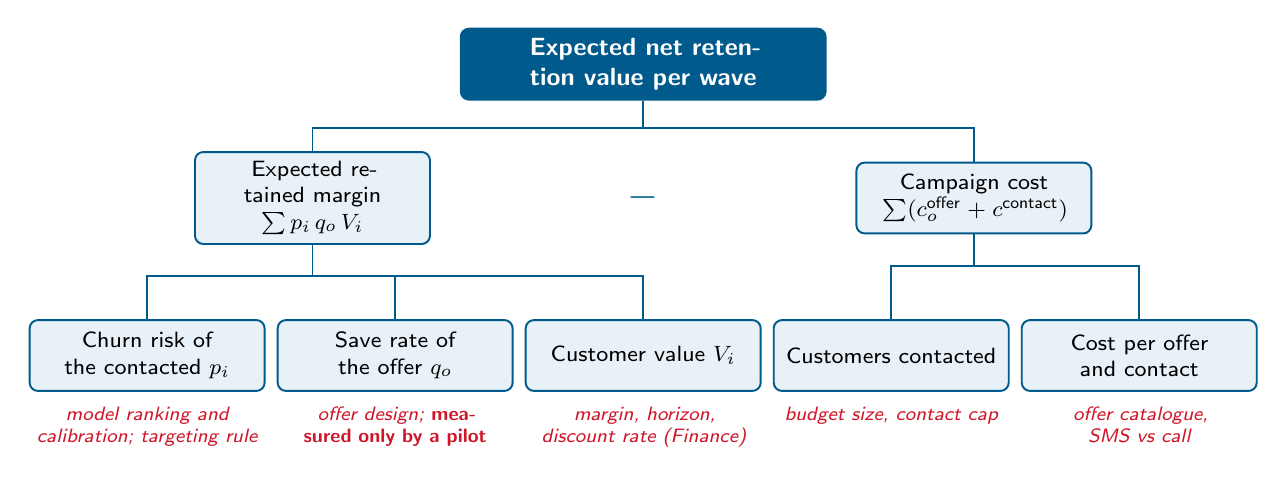
\begin{tikzpicture}[
  k/.style={draw=hustblue,fill=softblue,rounded corners=3pt,align=center,font=\footnotesize\sffamily,minimum height=0.9cm,text width=2.75cm,line width=0.7pt},
  top/.style={k,fill=hustblue,text=white,text width=4.4cm,font=\small\sffamily\bfseries},
  lev/.style={font=\scriptsize\sffamily\itshape,text=hustred,align=center,text width=2.8cm},
  e/.style={hustblue,line width=0.7pt}]
\node[top] (n) at (0,0) {Expected net retention value per wave};
\node[k] (r) at (-4.2,-1.7) {Expected retained margin\\$\sum p_i\, q_o\, V_i$};
\node[k] (c) at (4.2,-1.7) {Campaign cost\\$\sum (c^{\text{offer}}_o + c^{\text{contact}})$};
\node[font=\Large\bfseries,text=hustblue] at (0,-1.7) {$-$};
\node[k] (p) at (-6.3,-3.7) {Churn risk of the contacted $p_i$};
\node[k] (s) at (-3.15,-3.7) {Save rate of the offer $q_o$};
\node[k] (v) at (0,-3.7) {Customer value $V_i$};
\node[k] (nn) at (3.15,-3.7) {Customers contacted};
\node[k] (oc) at (6.3,-3.7) {Cost per offer and contact};
\draw[e] (n.south)--++(0,-0.35)-|(r.north); \draw[e] (n.south)--++(0,-0.35)-|(c.north);
\foreach \x in {p,s,v} \draw[e] (r.south)--++(0,-0.4)-|(\x.north);
\foreach \x in {nn,oc} \draw[e] (c.south)--++(0,-0.4)-|(\x.north);
\node[lev,below=2pt of p] {model ranking and calibration; targeting rule};
\node[lev,below=2pt of s] {offer design; \textbf{measured only by a pilot}};
\node[lev,below=2pt of v] {margin, horizon, discount rate (Finance)};
\node[lev,below=2pt of nn] {budget size, contact cap};
\node[lev,below=2pt of oc] {offer catalogue, SMS vs call};
\end{tikzpicture}
\caption{KPI tree of a retention campaign wave. Red text: the lever that moves each driver.}
\label{fig:kpitree}
\end{figure}

\textbf{Leading and lagging indicators.} Precision among contacted customers and coverage of high-risk/high-value customers are \emph{leading} indicators available as soon as a list is drawn. The realised save rate and net value per customer are \emph{lagging}: they appear only after the outcome window, by comparing offered customers with a randomised hold-out group.

\subsection{Success criteria, constraints and assumptions}

\begin{itemize}
  \item \textbf{Technical success:} PR-AUC and ROC-AUC clearly above the prior-only baseline on held-out data, with good calibration (expected calibration error below 0.05 and calibration slope near 1), because expected value multiplies a probability by money.
  \item \textbf{Business success:} at the same budget, the recommended rule must deliver a higher expected net value than the current highest-risk rule, and the advantage must survive the sensitivity analysis.
  \item \textbf{Constraints:} fixed budget per wave (base case: enough to give the standard offer to 10\% of customers, i.e.\ \$3,500 for the 1,409 test customers); one offer per customer; offer eligibility rules; contact cap of 30\%.
  \item \textbf{Assumptions:} offer save rates, offer and contact costs, contribution margin, value horizon and discount rate are \emph{visible parameters} with documented sources and tested ranges (Section~\ref{sec:assumptions}). The brief explicitly allows a synthetic offer-cost/response table; we never treat it as measured.
\end{itemize}

% ================================================================ 3
\section{Data Understanding and Preparation}

\subsection{Source and provenance}

The primary dataset is the IBM Telco Customer Churn sample distributed on Kaggle \cite{kaggle2018}: 7,043 customers of a \emph{fictional} US telco, 21 columns, one row per customer. The pipeline downloads it from Kaggle (with the IBM GitHub copy as a fallback), verifies its SHA-256 checksum (\texttt{88be4b93fbe0cc83\ldots}) and refuses to overwrite raw data that does not match. The file was downloaded on 2026-10-03; Kaggle lists version 1, last updated 2018-02-23. A second source, IBM's extended version of the same sample \cite{kaggle2020ibm}, is joined one-to-one on customer ID only to \emph{describe} why customers left; its fields never enter the model (Section~\ref{sec:leakage}).

\begin{table}[H]
\centering\small
\caption{Data dictionary (grouped). Full dictionary: \texttt{docs/data-dictionary.md}.}\label{tab:dict}
\begin{tabularx}{\linewidth}{@{}p{3.0cm}Xp{3.6cm}@{}}
\toprule
\textbf{Group} & \textbf{Fields} & \textbf{Use} \\
\midrule
Key & customerID & join key only \\
Demographics & gender, SeniorCitizen, Partner, Dependents & gender and SeniorCitizen: fairness audit only; Partner, Dependents: model inputs \\
Account & tenure (months), Contract, PaperlessBilling, PaymentMethod & model inputs; tenure also drives the value horizon \\
Charges & MonthlyCharges, TotalCharges & MonthlyCharges: input and value; TotalCharges dropped (collinear) \\
Services & PhoneService, MultipleLines, InternetService, OnlineSecurity, OnlineBackup, DeviceProtection, TechSupport, StreamingTV, StreamingMovies & model inputs; eligibility of the service-bundle offer \\
Target & Churn (Yes/No) & label; 1,869 churners (26.5\%) \\
\bottomrule
\end{tabularx}
\end{table}

\subsection{Data quality scorecard}

The course's data-quality dimensions were checked by an explicit schema in code; any violation stops the pipeline with the row and column that failed (Table~\ref{tab:dq}).

\begin{table}[H]
\centering\small
\caption{Data quality checks on the raw file.}\label{tab:dq}
\begin{tabularx}{\linewidth}{@{}p{2.6cm}Xp{4.6cm}@{}}
\toprule
\textbf{Dimension} & \textbf{Check} & \textbf{Result} \\
\midrule
Completeness & missing values per column & only \texttt{TotalCharges}: 11 blanks \\
Uniqueness & exact duplicate rows; duplicate IDs & 0 duplicates; 7,043 unique IDs \\
Validity & domains of every categorical field; numbers finite and non-negative; integer tenure & all values valid \\
Consistency & ``No internet service'' if and only if InternetService = No; ``No phone service'' if and only if PhoneService = No & no contradictions \\
Provenance & source URL, download time, SHA-256, licence note & recorded in \texttt{data/raw/source.json} \\
Cross-source agreement & extended sample: customer ID, churn label and shared fields & 7,043 of 7,043 customers matched, all shared fields agree \\
\bottomrule
\end{tabularx}
\end{table}

\textbf{Cleaning decisions.} The 11 blank \texttt{TotalCharges} values all belong to customers with \texttt{tenure} = 0, i.e.\ customers who have not yet received a bill. The values are missing for a structural reason (not at random), so they were set to 0 instead of being imputed with a mean. No other rows were filtered. Remaining missing numeric inputs in uploaded files are imputed with \emph{training-split} medians inside the model pipeline, so no information from the validation or test customers leaks into training.

\subsection{Validation design}

The sample is a single cross-sectional snapshot with no dates, so a temporal hold-out is impossible. We therefore used a stratified random split into train / validation / test = 4,225 / 1,409 / 1,409 customers (60/20/20, churn rate preserved in each part). Every choice (features, hyper-parameters, calibration, model, decision threshold, offer strategy, risk/value cut-offs and the budget) was made on train or validation; the test split was used once for reporting. Because each customer appears exactly once, there is no repeated-entity leakage between splits. With real operator data, the split should become temporal (train on earlier months, test on a later month); this is listed as a deployment requirement.

\subsection{Leakage audit}\label{sec:leakage}

Only information available at the scoring date may be used. Table~\ref{tab:leak} lists every field that was excluded and why.

\begin{table}[H]
\centering\small
\caption{Leakage and exclusion audit.}\label{tab:leak}
\begin{tabularx}{\linewidth}{@{}p{3.8cm}X@{}}
\toprule
\textbf{Field} & \textbf{Decision and reason} \\
\midrule
Churn reason, churn category (extended sample) & \textbf{Excluded.} Recorded only after a customer has left: target leakage. Used for description only. \\
IBM churn score, churn value (extended sample) & \textbf{Excluded.} IBM's own model output or the label itself. \\
CLTV index (extended sample) & \textbf{Excluded} from the model; used only to cross-check our value proxy. \\
TotalCharges & \textbf{Dropped} by the feature review: it is almost exactly tenure $\times$ monthly charges, adds no cross-validated precision and makes coefficients unstable (multicollinearity). \\
gender, SeniorCitizen & \textbf{Excluded} as model inputs on fairness grounds; kept for the allocation audit. \\
customerID & \textbf{Excluded}: an identifier, not a behaviour. \\
\bottomrule
\end{tabularx}
\end{table}

A known limitation of this teaching sample remains: tenure, contract and charges are observed in the same snapshot as the churn flag, so for churners they describe the customer at departure. No feature is derived from the label itself, but with real data the inputs must be taken from a snapshot \emph{before} the outcome window.

% ================================================================ 4
\section{Exploratory Analysis: Who Churns and Who Is Worth Saving}

\subsection{Churn drivers}

Figure~\ref{fig:eda} shows observed churn by segment on the training split. Churn is highest for month-to-month contracts (43\% against 3\% on two-year contracts), new customers with tenure of 12 months or less (48\% against 14\% for customers with more than 24 months), fibre-optic internet (42\% against 7\% without internet) and payment by electronic check (46\% against 15\% for automatic credit-card payment). Customers without TechSupport (42\%) or OnlineSecurity (42\%) churn more than those with them. Senior citizens churn at 41\% against 24\%. These are associations in observational data, not causes: moving a customer to a two-year contract will not necessarily remove the risk that led the customer to choose a monthly one.

\begin{figure}[H]
\centering
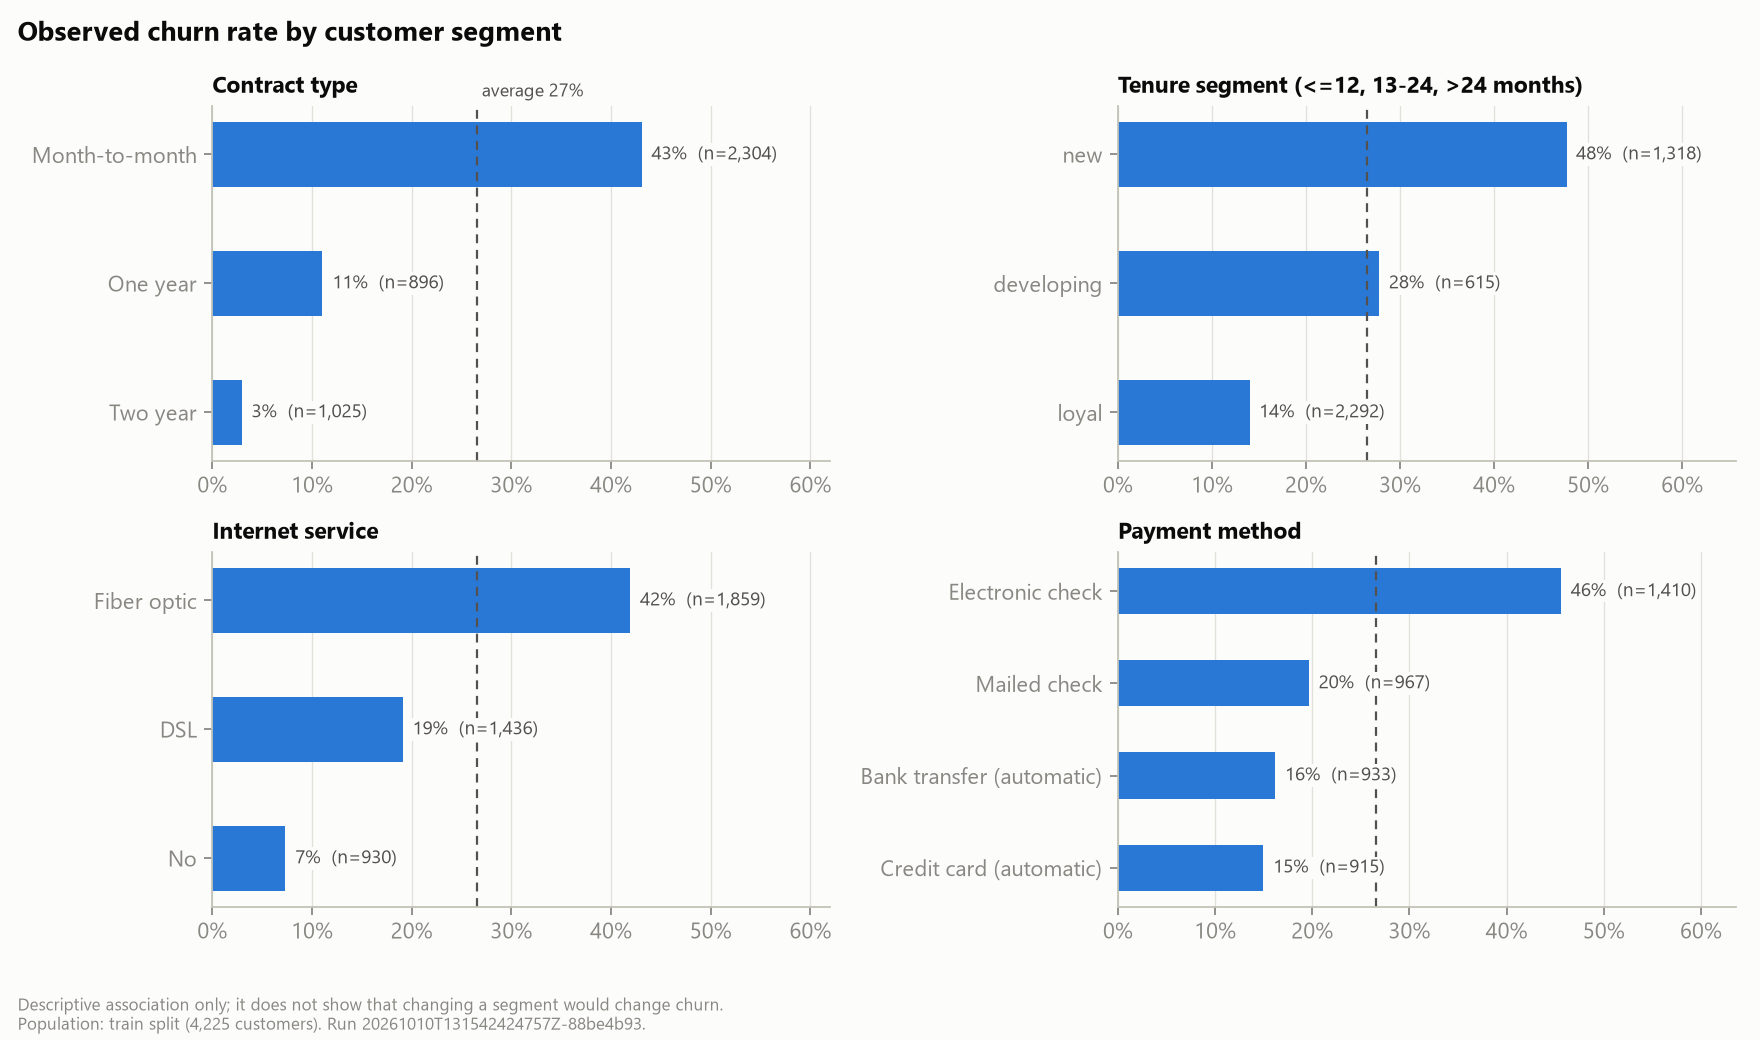
\includegraphics[width=0.95\linewidth]{eda_drivers.png}
\caption{Observed churn rate by segment (training split, 4,225 customers).}
\label{fig:eda}
\end{figure}

\subsection{Risk and value only partly overlap}

The key business insight of the EDA is that the customers most likely to leave are not the customers most worth keeping. Using the 75th percentiles of predicted risk (0.465) and customer value (\$345), fitted on validation and frozen, the test customers fall into four segments (Table~\ref{tab:quad}, Figure~\ref{fig:riskvalue}).

\begin{table}[H]
\centering\small
\caption{Risk $\times$ value segments on the test split and how many customers each rule contacts at the base budget.}\label{tab:quad}
\begin{tabularx}{\linewidth}{@{}Lrrrrrr@{}}
\toprule
\textbf{Segment} & \hd{Customers} & \hd{Observed\\churn} & \hd{Mean\\value} & \hd{Share of value\\at risk} & \hd{Contacted:\\risk-only} & \hd{Contacted:\\recommended} \\
\midrule
High risk / High value & 57 & 54.4\% & \$402 & 13.7\% & 7 & 56 \\
High risk / Low value & 306 & 59.8\% & \$221 & 46.1\% & 133 & 85 \\
Low risk / High value & 291 & 19.2\% & \$414 & 20.9\% & 0 & 12 \\
Low risk / Low value & 755 & 13.8\% & \$164 & 19.2\% & 0 & 0 \\
\bottomrule
\end{tabularx}
\end{table}

The high-risk/low-value segment holds the largest share of value at risk (46\%), but each of its customers is worth little; the risk-only rule spends almost its whole budget there. The recommended rule reaches 56 of the 57 high-risk/high-value customers and adds valuable customers at moderate risk.

\begin{figure}[H]
\centering
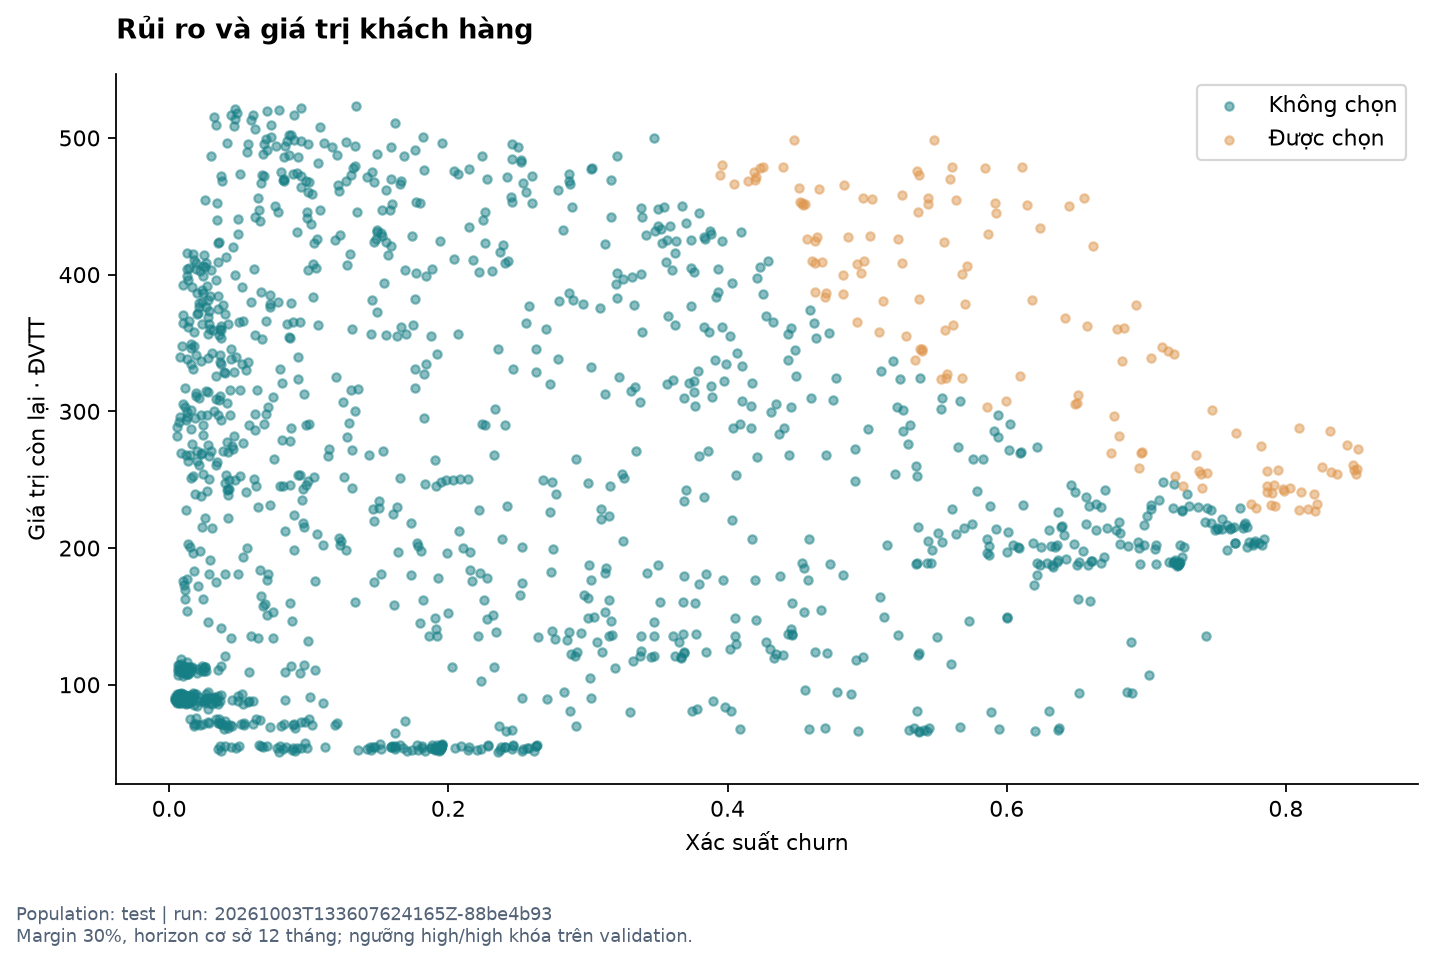
\includegraphics[width=0.82\linewidth]{risk_value.png}
\caption{Risk $\times$ value map of the test customers. Dashed lines: 75th percentiles fitted on validation.}
\label{fig:riskvalue}
\end{figure}

\subsection{Why customers leave}

IBM's extended sample records a reason for each of the 1,869 churners. Reasons are known only after departure, so they are used to understand what an offer \emph{can} fix, not to predict (Table~\ref{tab:reasons}). Only 46\% of churners left for price or a competitor's offer; 42\% cite staff attitude or dissatisfaction with the network, product or support, which call for service fixes rather than discounts. This bounds the assumed save rate: if an offer can only reach the addressable churners, a 20\% save rate means keeping about 43\% of those it can reach, an ambitious figure that must be tested. The most frequent single reason is ``Attitude of support person'' (10\% of churners).

\begin{table}[H]
\centering\small
\caption{Churn reason categories (IBM grouping).}\label{tab:reasons}
\begin{tabularx}{0.85\linewidth}{@{}Lrrl@{}}
\toprule
\textbf{Category} & \hd{All\\churners} & \hd{Churners on the\\recommended list} & \textbf{Addressable by an offer?} \\
\midrule
Competitor & 33\% & 33\% & Yes \\
Dissatisfaction & 25\% & 27\% & No \\
Attitude & 17\% & 16\% & No \\
Price & 13\% & 13\% & Yes \\
Other & 11\% & 10\% & No \\
\bottomrule
\end{tabularx}
\end{table}

% ================================================================ 5
\section{Modelling Churn Risk}

\subsection{Candidates, tuning and selection}

Three model families were trained on the same inputs: \textbf{logistic regression} (the interpretable baseline), a \textbf{random forest} (the required tree-based model) and \textbf{XGBoost} gradient boosting (stretch). Each was tuned by 5-fold stratified cross-validation on the training split with average precision (PR-AUC) as the objective, because churners are a minority and the business cares about the top of the ranking \cite{saito2015}. Each tuned model was then calibrated with a sigmoid (Platt) mapping fitted on out-of-fold predictions \cite{platt1999,niculescu2005}. A prior-only model, which predicts the churn rate for everyone, anchors the metrics.

\textbf{Feature design.} Before tuning, a cross-validated review on the training split compared four candidate feature sets. The rule, fixed in advance, was: \emph{full-rank sets only; cross-validated ap within one standard error of the best full-rank candidate; then the fewest encoded columns}. It selected the set ``without TotalCharges'' (Table~\ref{tab:ablation}). Categorical variables are coded against their lowest-churn level (for example, two-year contracts), which avoids the dummy-variable trap and lets odds ratios read ``compared with\ldots''.

\begin{table}[H]
\centering\small
\caption{Cross-validated feature review (training split, logistic regression).}\label{tab:ablation}
\begin{tabularx}{\linewidth}{@{}Lrrrl@{}}
\toprule
\textbf{Feature set} & \hd{CV\\PR-AUC} & \hd{Std.\\error} & \hd{Encoded\\columns} & \textbf{Full rank} \\
\midrule
all inputs & 0.664 & 0.014 & 21 & yes \\
\winrow without TotalCharges (selected) & 0.661 & 0.013 & 20 & yes \\
without TotalCharges, with tenure band & 0.664 & 0.013 & 22 & yes \\
all inputs with tenure band & 0.665 & 0.014 & 23 & yes \\
previous design (reference) & 0.665 & 0.013 & 48 & no \\
\bottomrule
\end{tabularx}
\end{table}

\textbf{Selection rule} (validation, fixed in advance): \emph{AP within 0.01 of best calibrated candidate; Brier within 0.002 of best; prefer simpler}. Tree models did not rank customers better than logistic regression, so the calibrated \textbf{logistic regression} was deployed.

\subsection{Performance on the held-out test split}

\begin{table}[H]
\centering\small
\caption{Test performance (1,409 customers). Recall is at the F1-optimal threshold chosen on validation (0.40).}\label{tab:test}
\begin{tabularx}{\linewidth}{@{}Lrrrrrr@{}}
\toprule
\textbf{Model} & \hd{PR-AUC} & \hd{ROC-AUC} & \hd{Brier} & \hd{ECE} & \hd{Cal.\ slope} & \hd{Recall} \\
\midrule
Prior-only baseline & 0.265 & 0.500 & 0.195 & 0.022 & n/a & 0\% \\
Logistic regression & 0.620 & 0.830 & 0.142 & 0.021 & 0.92 & 65\% \\
\winrow Logistic regression, calibrated & 0.620 & 0.830 & 0.142 & 0.019 & 0.94 & 65\% \\
Random forest & 0.621 & 0.832 & 0.141 & 0.020 & 1.05 & 62\% \\
Random forest, calibrated & 0.621 & 0.832 & 0.144 & 0.045 & 0.91 & 59\% \\
XGBoost & 0.613 & 0.826 & 0.144 & 0.026 & 0.84 & 63\% \\
XGBoost, calibrated & 0.613 & 0.826 & 0.145 & 0.044 & 0.93 & 57\% \\
\bottomrule
\end{tabularx}
\end{table}

The deployed model reaches a PR-AUC of 0.620 (bootstrap 95\% interval 0.567--0.671) against a baseline of 0.265, and a ROC-AUC of 0.830 (0.807--0.851). The riskiest decile churns at 71\% (lift 2.67), and the top three deciles capture 64\% of all churners. Test PR-AUC is lower than on validation (0.672), and the validation value lies outside the test interval: validation was used to choose among candidates, so its score is optimistic, and the test figure is the one to rely on.

\begin{figure}[H]
\centering
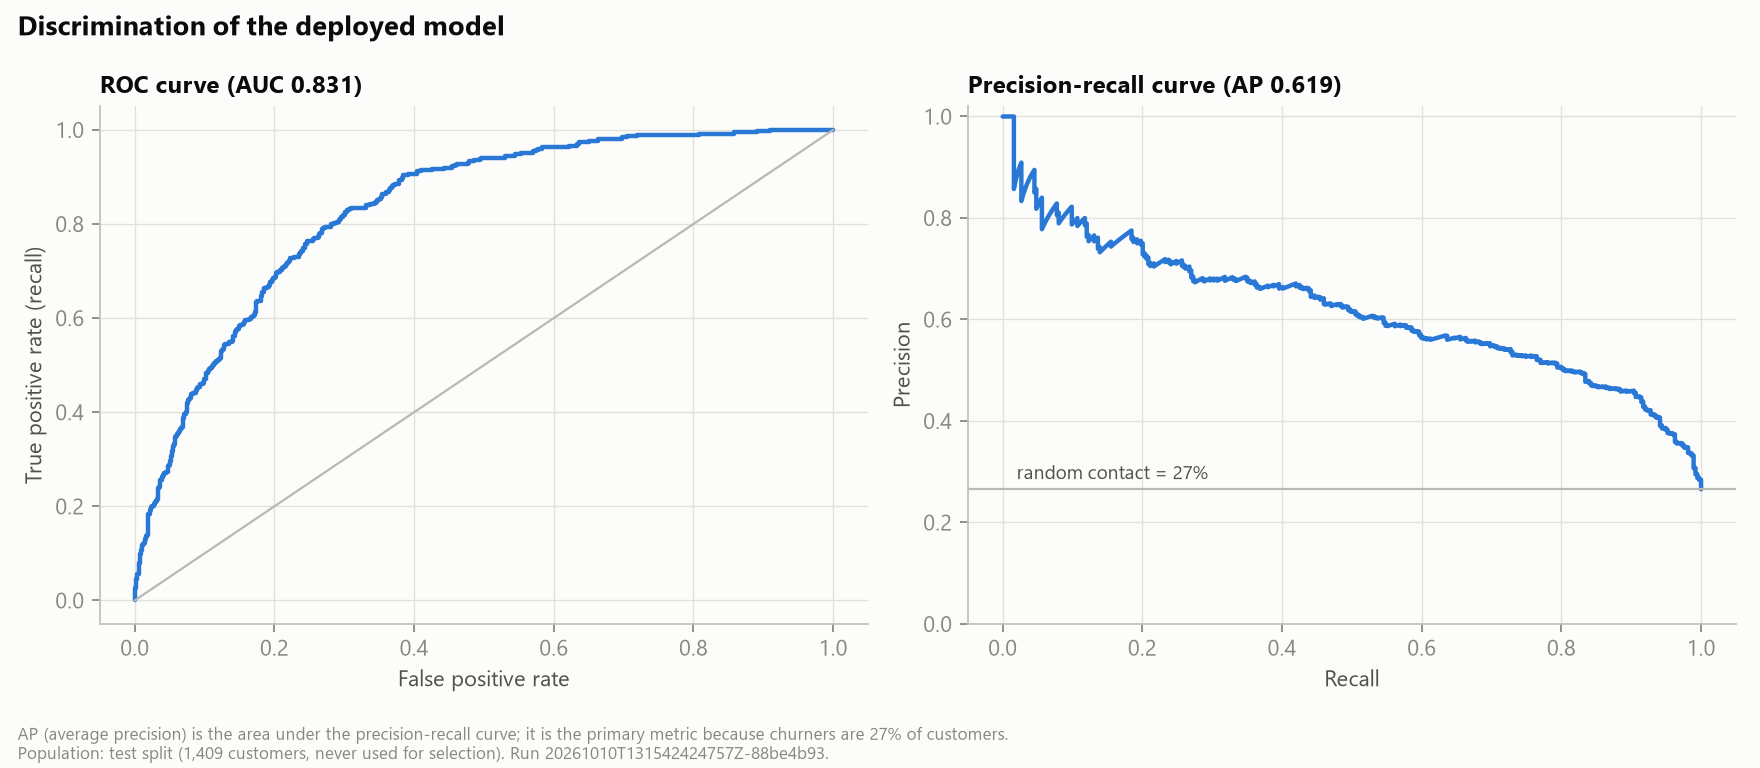
\includegraphics[width=0.49\linewidth]{discrimination.png}\hfill
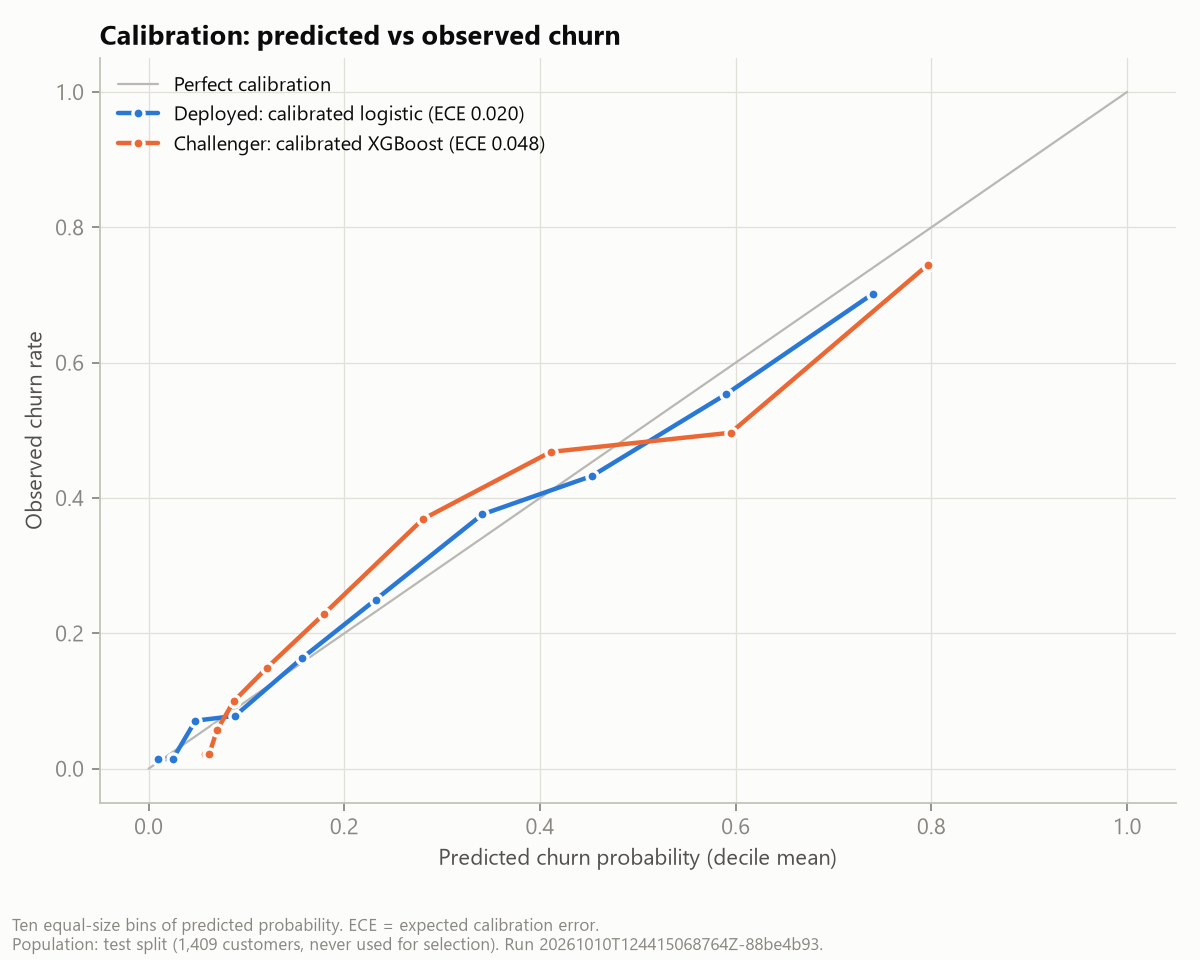
\includegraphics[width=0.49\linewidth]{calibration.png}
\caption{Left: discrimination (ROC and precision--recall) of the deployed model. Right: reliability curve on ten equal-size bins of predicted probability (test split).}
\label{fig:model}
\end{figure}

\textbf{Calibration matters as much as ranking.} Expected value multiplies a probability by money, so a model that ranks well but over-states risk would over-spend. The deployed model's expected calibration error is 0.019 \cite{guo2017}, its calibration slope 0.94 (target 1) and intercept \textminus{}0.032 (target 0) \cite{vancalster2019}. Sigmoid calibration made little difference to logistic regression and \emph{worsened} the tree models' ECE on test; we report this as found.

\textbf{The model choice checked in money.} At the base budget, the three calibrated models produce similar expected value on test, but valued with customers' actual churn the logistic list is worth \$1,977 against \$1,591 for the random forest and \$1,468 for XGBoost: the simpler model is not a sacrifice.

\subsection{What drives predicted churn}

Figure~\ref{fig:drivers} shows the odds ratios of the deployed logistic model. Holding the other inputs fixed, a month-to-month contract multiplies the odds of churn by 3.66 compared with a two-year contract, and fibre internet by 2.90 compared with no internet. Longer tenure lowers the odds (by a factor of 0.69 per 12 months), as do phone service, OnlineSecurity and TechSupport. The XGBoost challenger, explained with TreeSHAP \cite{lundberg2017}, ranks the same drivers first (Contract\_Month-to-month, tenure, MonthlyCharges, InternetService\_Fiber optic), which increases confidence that the drivers are stable across model families. Both are associations, not causal effects.

\begin{figure}[H]
\centering
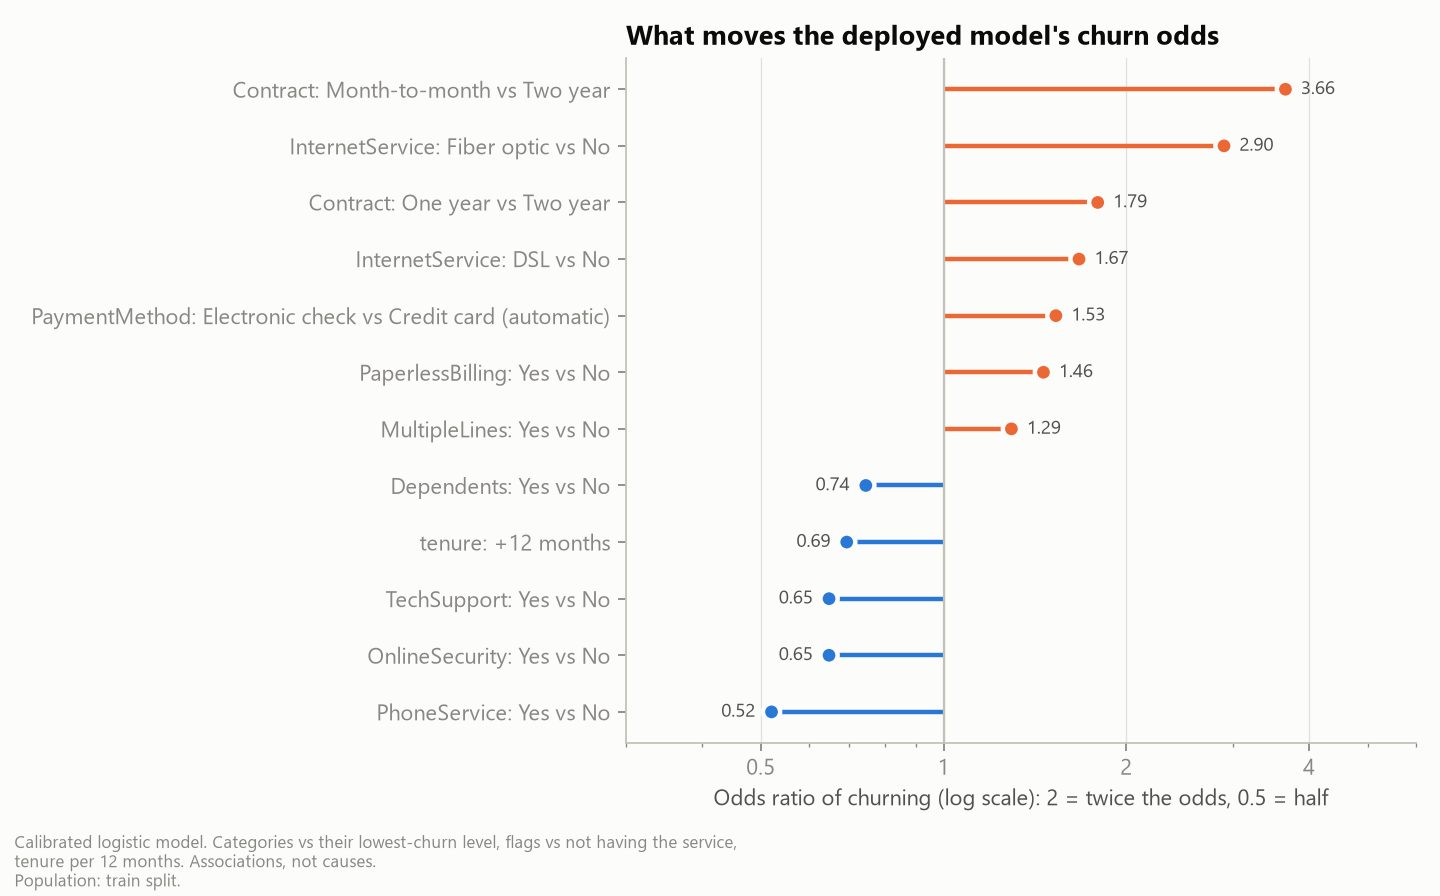
\includegraphics[width=0.53\linewidth]{model_drivers.png}\hfill
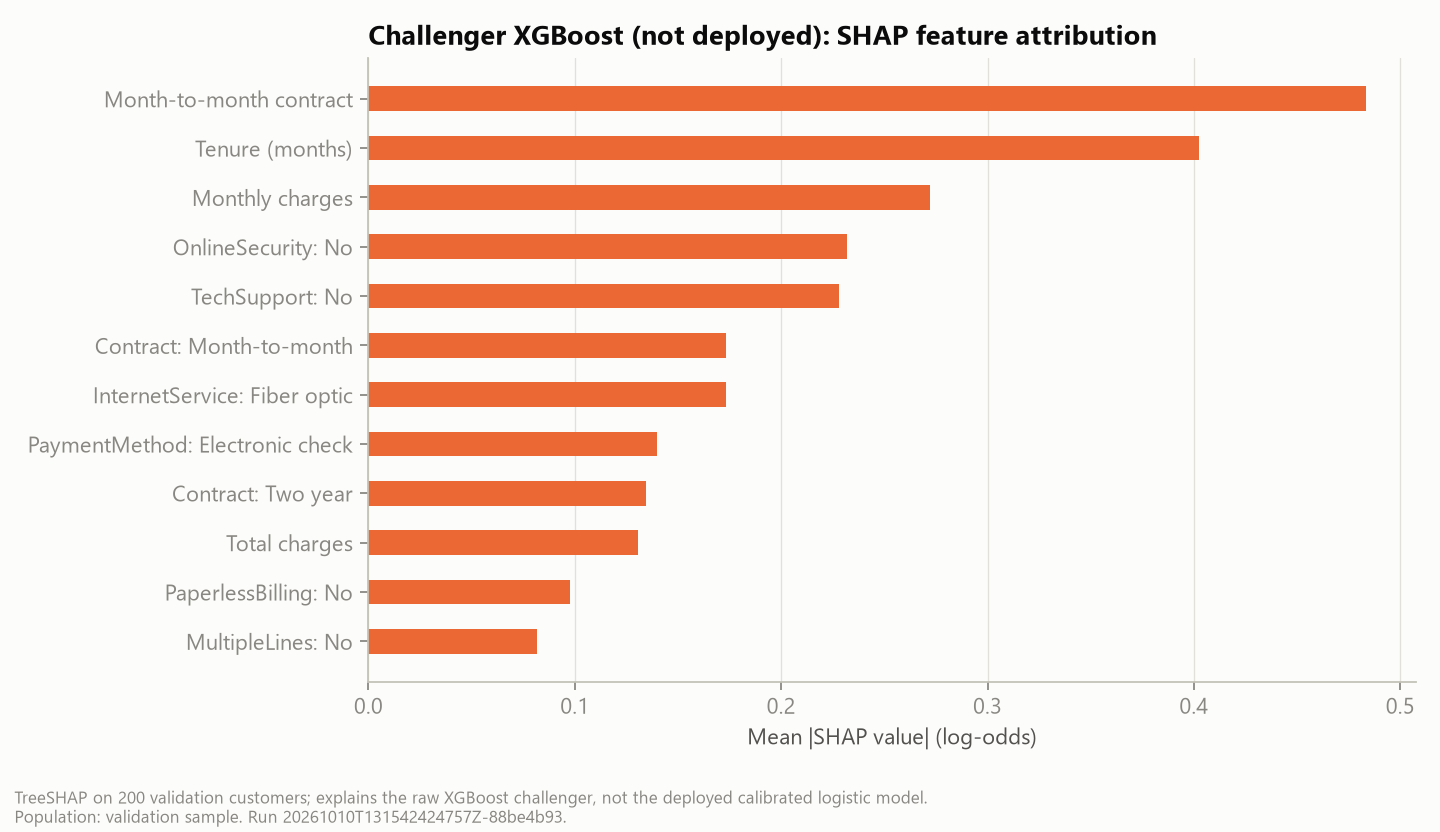
\includegraphics[width=0.45\linewidth]{shap_challenger.png}
\caption{Left: odds ratios of the deployed model (categories against their lowest-churn level, tenure per 12 months). Right: mean absolute SHAP values of the XGBoost challenger on 200 validation customers.}
\label{fig:drivers}
\end{figure}

\textbf{Points scorecard.} For the call centre, the logistic model is also published as a points card (base 133 points; every 40 points double the odds of churn). On test the card reproduces the model's probability within 1.0 percentage points on average and has the same ROC-AUC (0.831), so agents can explain a score without software (\texttt{docs/churn-scorecard.md}).

\textbf{Error analysis.} At the F1 threshold, false positives (191 customers flagged who stayed) look like true churners: 99\% month-to-month and 80\% fibre. Missed churners (132) have longer tenure (mean 31 months) and lower bills, i.e.\ customers whose departure the snapshot does not foreshadow. The weakest segment for ranking is month-to-month contracts (ROC-AUC 0.74), because almost all of them are risky; calibration is weakest for senior citizens (ECE 0.049 against 0.019), which is followed up in the fairness audit.

% ================================================================ 6
\section{From Prediction to Decision}

\subsection{Customer value proxy}

The data contain no margin or lifetime, so value is a transparent proxy built from tenure and charges, as the brief suggests:
\begin{gather*}
V_i \;=\; \text{MonthlyCharges}_i \times m \times a\!\left(H_i, r\right),\
H_i = \min\!\big(H_{\max},\, H_0 \cdot f_{\text{seg}(i)}\big),\\
a(H,r) = \frac{1-(1+r_m)^{-H}}{r_m},
\end{gather*}
with contribution margin $m$ = 30\%, base horizon $H_0$ = 12 months scaled by tenure segment ($f$ = 0.75 / 1.0 / 1.25 for new / developing / loyal customers), cap $H_{\max}$ = 24 months and a 10\% annual discount rate ($r_m$ is the equivalent monthly rate). It is a deliberately short, truncated value \cite{faderhardie2014,gupta2004}: a saved would-be churner is likely to leave again sooner than an average customer. As a sanity check, its rank correlation with IBM's CLTV index is only 0.18, because that index is driven by tenure (0.37) whereas our proxy measures the \emph{next} months of margin at stake.

\subsection{Expected value of an offer and the decision rule}

For customer $i$ and offer $o$:
\[
\text{EV}_{i,o} \;=\; \underbrace{p_i}_{\text{churn risk}} \times \underbrace{q_o}_{\text{save rate}} \times \underbrace{V_i}_{\text{value}} \;-\; \big(\underbrace{c^{\text{offer}}_o + c^{\text{contact}}}_{\text{cost}}\big).
\]
The offer cost is charged to every contacted customer (an unconditional credit), which is conservative. A customer is worth contacting only when $\text{EV} > 0$; equivalently, the customer's churn probability must exceed the \emph{break-even probability} $c/(q\,V_i)$, which depends on the customer's value. On test this break-even probability ranges from 29\% for the most valuable decile to above 100\% (never worth an offer) for the least valuable ones, which is why a single probability threshold cannot be right.

\keybox{hustblue}{\textbf{Worked example.} A customer pays \$70 a month and has 20 months of tenure (``developing'', 12-month horizon). Discounted, the horizon is worth 11.40 months of margin, so $V$ = \$70 $\times$ 30\% $\times$ 11.40 = \$239.41. With $p$ = 0.60, the standard offer ($q$ = 20\%, cost \$25) gives EV = 0.60 $\times$ 0.20 $\times$ \$239.41 $-$ \$25 = \$3.73: barely worth it. At this risk the customer would need a value of at least \$208.33 to break even.}

\textbf{Offer catalogue.} The brief allows a synthetic, documented offer table. Four offers with eligibility rules were defined (Table~\ref{tab:offers}); their costs and save rates are team assumptions to be replaced by pilot measurements.

\begin{table}[H]
\centering\small
\caption{Synthetic offer catalogue (assumptions, not measurements).}\label{tab:offers}
\begin{tabularx}{\linewidth}{@{}Lrrrp{4.3cm}@{}}
\toprule
\textbf{Offer} & \hd{Offer\\cost} & \hd{Contact\\cost} & \hd{Save\\rate} & \textbf{Eligibility} \\
\midrule
One-time \$20 bill credit & \$20 & \$5 & 20\% & All customers \\
\$35 credit for moving to a 1-year contract & \$35 & \$5 & 30\% & Contract: Month-to-month \\
6 months free TechSupport + OnlineSecurity & \$12 & \$5 & 15\% & InternetService: DSL or Fiber optic; TechSupport: No \\
\$10 loyalty reward & \$10 & \$5 & 10\% & tenure\_segment: loyal \\
\bottomrule
\end{tabularx}
\end{table}

\subsection{Budget-constrained optimisation}

Choosing customers and offers within a budget is a knapsack problem. With binary decision $x_{i,o}$ (customer $i$ receives offer $o$), budget $B$, $N$ customers and contact cap $\kappa$:
\[
\max_{x}\; \sum_{i,o} \text{EV}_{i,o}\, x_{i,o}
\quad\text{s.t.}\quad
\sum_{o} x_{i,o} \le 1 \;\;\forall i,\qquad
\sum_{i,o} \big(c^{\text{offer}}_o + c^{\text{contact}}\big)\, x_{i,o} \le B,\qquad
\sum_{i,o} x_{i,o} \le \kappa N,
\]
with $x_{i,o}=0$ when the customer is not eligible for the offer or $\text{EV}_{i,o}\le 0$. It is solved exactly as a mixed-integer program (SciPy/HiGHS, zero optimality gap); with a single offer and equal costs, sorting by EV is provably optimal and is used directly. Unit tests check the optimiser against brute force on small cases.

\subsection{Threshold rules versus expected value}

The baseline brief asks for threshold analysis. The F1-optimal threshold on validation is 0.40, but a threshold ignores value and cost (Table~\ref{tab:threshold}): contacting everyone above it costs more and earns less than contacting only customers with positive expected value.

\begin{table}[H]
\centering\small
\caption{Probability threshold versus expected-value rules (standard offer, test split).}\label{tab:threshold}
\begin{tabularx}{\linewidth}{@{}Lrrrrr@{}}
\toprule
\textbf{Rule} & \hd{Customers} & \hd{Cost} & \hd{Expected\\net value} & \hd{Precision} & \hd{Recall} \\
\midrule
Probability >= 0.40 (F1 threshold) & 433 & \$10,825 & \$1,989 & 55.9\% & 64.7\% \\
Expected value > 0 (no budget limit) & 332 & \$8,300 & \$3,202 & 56.3\% & 50.0\% \\
Expected value, ranked within the fixed budget & 140 & \$3,500 & \$2,340 & 60.0\% & n/a \\
\bottomrule
\end{tabularx}
\end{table}

% ================================================================ 7
\section{Results: Targeting at a Fixed Budget}

\subsection{Strategy comparison}

All rules receive the same budget (\$3,500, enough for the standard offer to 10\% of the 1,409 test customers). Table~\ref{tab:strategies} and Figure~\ref{fig:strategies} compare them. ``Label-based net'' revalues each frozen list with customers' \emph{actual} churn instead of predicted probabilities (still at the assumed save rates).

\begin{table}[H]
\centering\small
\caption{Strategies at the same budget on the test split. HR/HV = high-risk/high-value customers.}\label{tab:strategies}
\setlength{\tabcolsep}{4pt}
\begin{tabularx}{\linewidth}{@{}Lrrrrrrr@{}}
\toprule
\textbf{Rule} & \hd{Con-\\tacted} & \hd{Cost} & \hd{Expected\\net value} & \hd{ROI} & \hd{Preci-\\sion} & \hd{HR/HV\\coverage} & \hd{Label-\\based net} \\
\midrule
No campaign & 0 & \$0 & \$0 & n/a & n/a & 0\% & \$0 \\
Highest churn risk & 140 & \$3,500 & \$1,301 & 37\% & 71\% & 12\% & \$1,079 \\
Highest risk, positive EV only & 140 & \$3,500 & \$1,367 & 39\% & 69\% & 12\% & \$1,105 \\
Highest customer value & 140 & \$3,500 & \textminus{}\$1,037 & \textminus{}30\% & 29\% & 30\% & \$90 \\
Expected value (single offer) & 140 & \$3,500 & \$2,340 & 67\% & 60\% & 96\% & \$1,977 \\
\winrow Expected value + segment offers & 153 & \$3,500 & \$2,668 & 76\% & 60\% & 98\% & \$2,156 \\
Random contact (mean of runs) & 140 & \$3,500 & \textminus{}\$1,645 & \textminus{}47\% & 26\% & 10\% & \textminus{}\$1,688 \\
\bottomrule
\end{tabularx}
\end{table}

\begin{figure}[H]
\centering
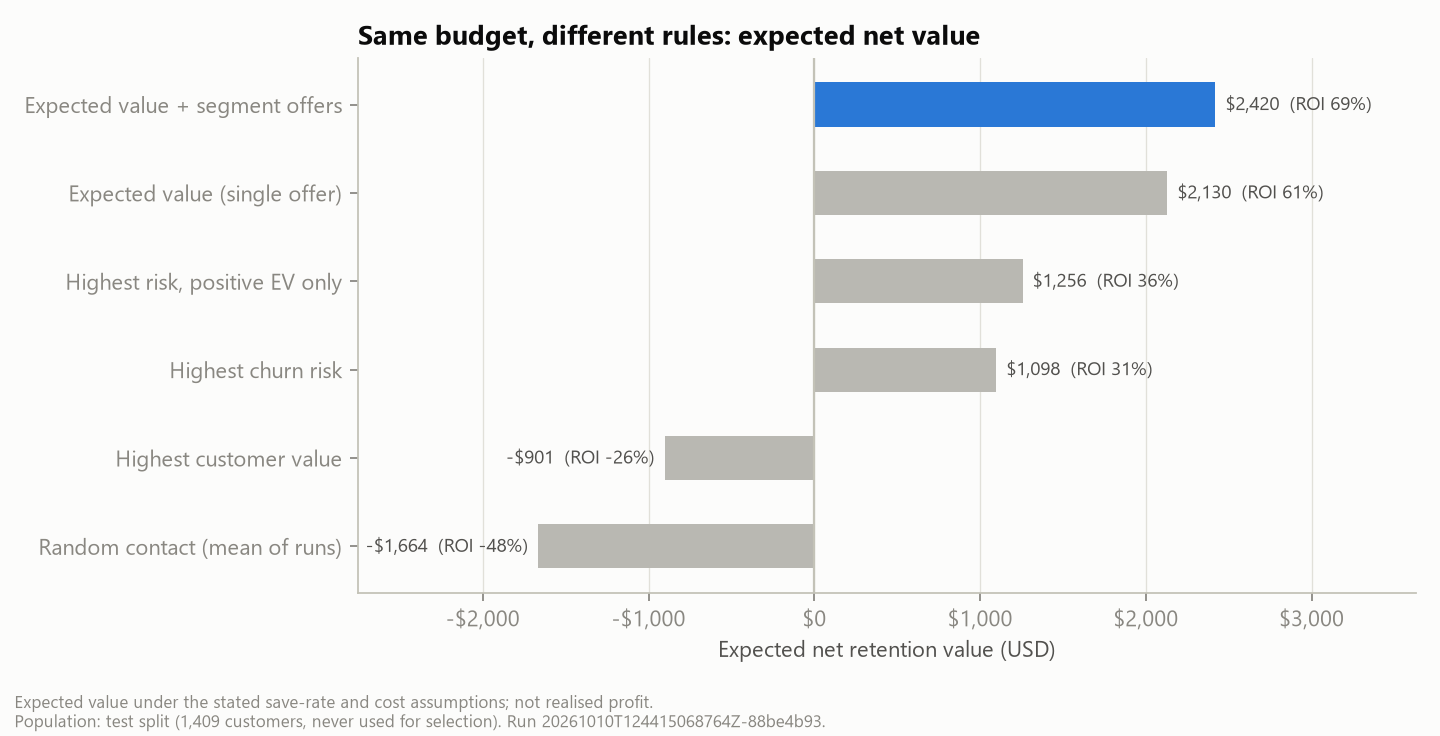
\includegraphics[width=0.85\linewidth]{strategy_comparison.png}
\caption{Expected net value of each rule at the same budget (test split). Expected values under the stated assumptions, not realised profit.}
\label{fig:strategies}
\end{figure}

\begin{itemize}
  \item \textbf{Targeting effect.} With the same standard offer, ranking by expected value instead of risk adds +\$1,039 of expected value; valued with actual churn it adds +\$898 (paired bootstrap 95\% interval \$107 to \$1,744), so the gain does not rest on the model's own probabilities.
  \item \textbf{Offer-design effect.} Matching offers to segments adds +\$328 expected (label-based +\$179, interval \textminus{}\$153 to \$577). This part comes from \emph{assumed} offer-specific save rates and is not proven; the pilot tests each offer as its own arm. On validation it beat the single offer by 13\%, above the 5\% rule fixed in advance, so it is the recommended rule.
  \item \textbf{Precision is not the goal.} Risk-only targeting is more precise (71\% vs 60\% of contacted customers churn) but spends on risky customers whose remaining value cannot repay an offer. The recommended rule covers 98\% of high-risk/high-value customers against 12\%.
  \item \textbf{Value alone and random contact lose money}, because offers to customers who would have stayed anyway are pure cost.
\end{itemize}

\subsection{Who receives an offer}

On the recommended list, 100\% of customers have fibre (44\% of all test customers), 97\% are on month-to-month contracts (56\%) and 73\% pay by electronic check (35\%); their mean predicted churn is 60\% against 27\% overall. The optimiser mixes the offers as follows: \$35 credit for moving to a 1-year contract (150 customers); 6 months free TechSupport + OnlineSecurity (150 customers); One-time \$20 bill credit (24 customers). The loyalty reward is never chosen under the current assumptions.

\begin{figure}[H]
\centering
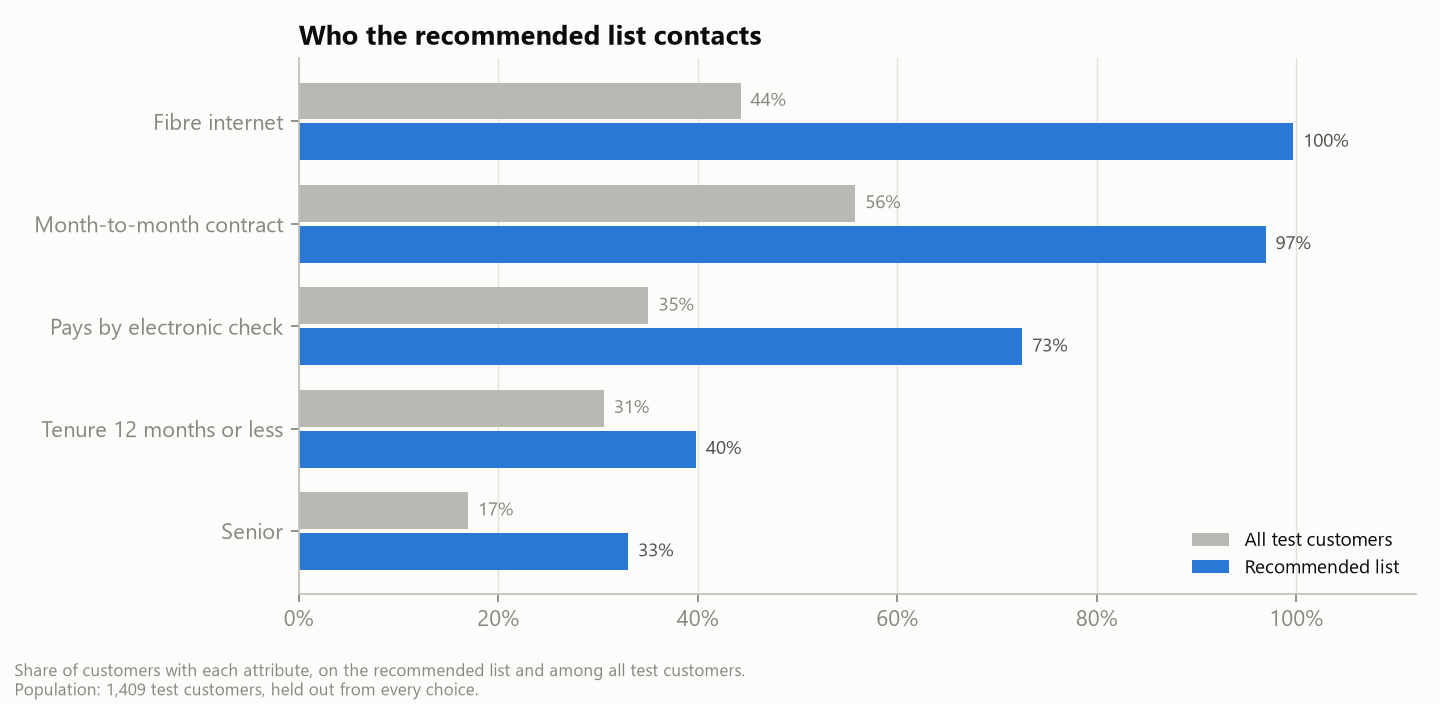
\includegraphics[width=0.49\linewidth]{target_profile.png}\hfill
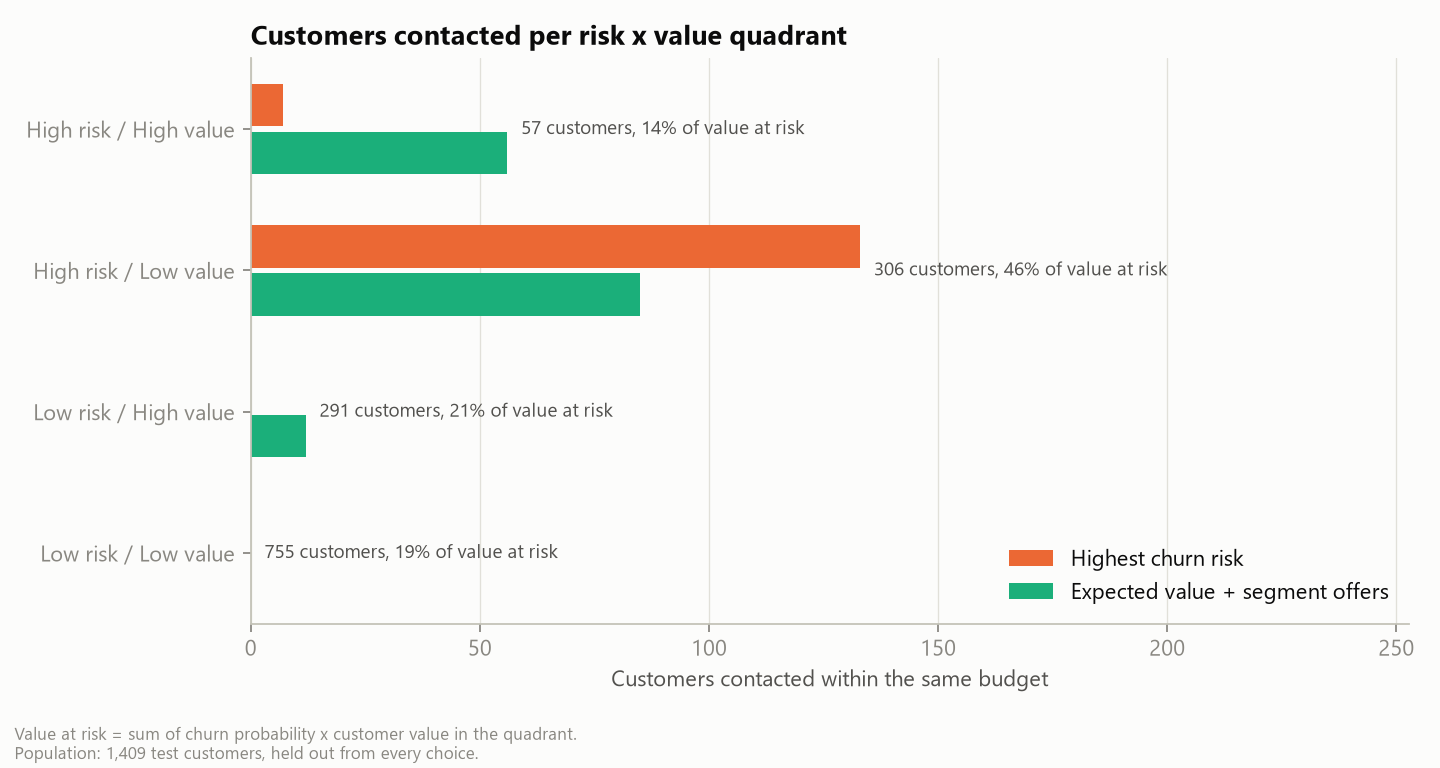
\includegraphics[width=0.49\linewidth]{quadrant_selection.png}
\caption{Left: profile of the recommended list against all test customers. Right: which risk/value segments each rule contacts.}
\label{fig:profile}
\end{figure}

\subsection{How much to spend: the profit curve}

Expected net value rises with the budget at a falling marginal return (Figure~\ref{fig:profit}). The budget rule, fixed before looking at test, is: \emph{take the largest budget whose last step still returns at least 10\% on its cost}. Applied on validation it chose 26\% (the net-maximising budget on validation was 32\%; the hurdle stops earlier because the last steps barely pay for themselves).

\begin{table}[H]
\centering\small
\caption{Base and recommended budgets on the test split.}\label{tab:budget}
\begin{tabularx}{\linewidth}{@{}Lrrrrr@{}}
\toprule
\textbf{Budget} & \hd{Contacted} & \hd{Cost} & \hd{Expected\\net value} & \hd{ROI} & \hd{Label-based\\net} \\
\midrule
Base (10\%) & 153 (11\%) & \$3,500 & \$2,668 & 76\% & \$2,156 \\
\winrow Recommended (26\%) & 324 (23\%) & \$9,150 & \$4,145 & 45\% & \$3,377 \\
\bottomrule
\end{tabularx}
\end{table}

Beyond 371 contacts on test (26\% of customers) no customer has a positive expected value, so extra budget should stay unspent. Scaled linearly to the 7,043-customer base, the recommended wave is about 1,620 customers and \$45,737 for \$20,721 of expected net value (indicative only).

\begin{figure}[H]
\centering
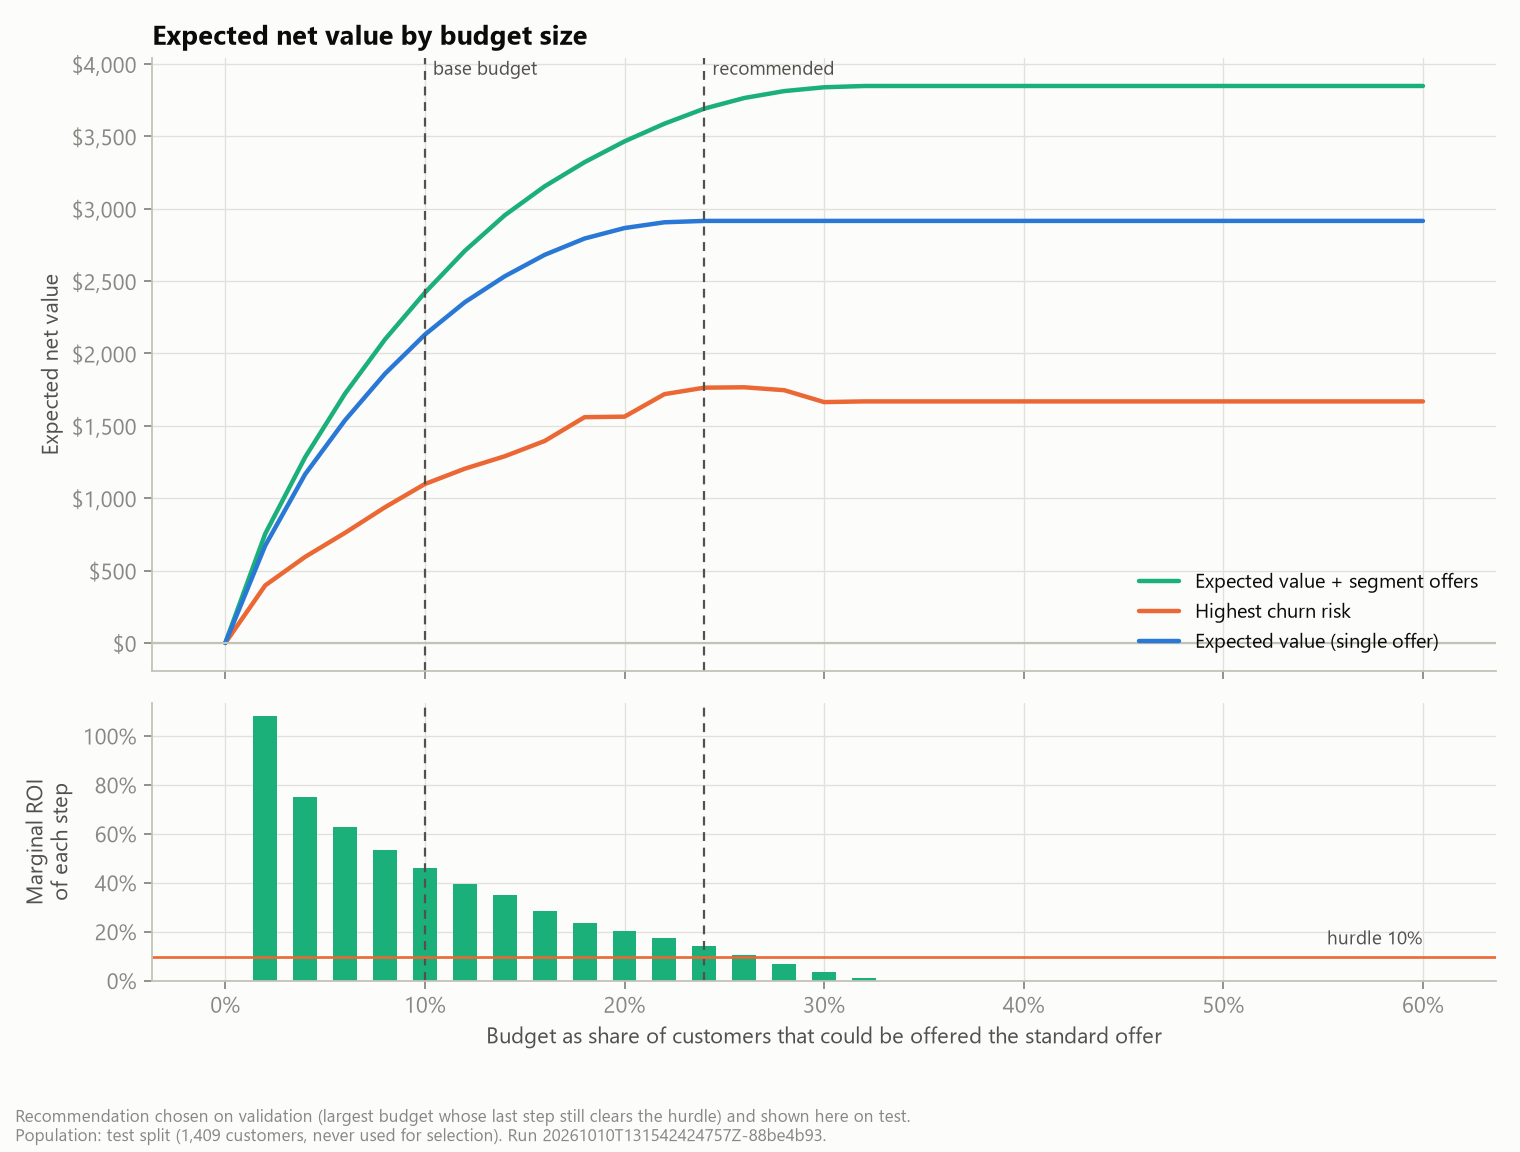
\includegraphics[width=0.85\linewidth]{profit_curve.png}
\caption{Profit curve and marginal ROI by budget (test split). The recommendation was chosen on validation.}
\label{fig:profit}
\end{figure}

% ================================================================ 8
\section{Robustness and Sensitivity}\label{sec:assumptions}

Every money figure depends on assumptions the data cannot measure. They are listed with sources and tested ranges in the assumption register (Table~\ref{tab:register}) and are adjustable in the dashboard.

\begin{table}[H]
\centering\small
\caption{Assumption register (base value and tested range).}\label{tab:register}
\begin{tabularx}{\linewidth}{@{}p{0.6cm}Lrrrp{4.4cm}@{}}
\toprule
\textbf{ID} & \textbf{Assumption} & \textbf{Low} & \textbf{Base} & \textbf{High} & \textbf{Validate by} \\
\midrule
A1 & Save rate of the standard offer & 10\% & 20\% & 30\% & Randomised holdout pilot (docs/pilot-design.md) \\
A2 & Offer cost (multiplier on catalog cost) & x0.5 & x1 & x1.5 & Finance sign-off of the offer budget \\
A3 & Contact cost per customer (USD) & \$1 & \$5 & \$10 & Call-centre cost per completed contact \\
A4 & Contribution margin & 20\% & 30\% & 40\% & Finance (product P\&L) \\
A5 & Value horizon (months) & 6 months & 12 months & 18 months & Survival of pilot customers after 6 and 12 months \\
A6 & Annual discount rate & 5\% & 10\% & 15\% & Finance hurdle rate \\
A7 & Tenure effect on remaining months (new 1-s, loyal 1+s) & 0\% & 25\% & 50\% & Survival of pilot customers by tenure segment \\
\bottomrule
\end{tabularx}
\end{table}

\subsection{One assumption at a time}

Each bar of the tornado chart (Figure~\ref{fig:tornado}) moves one assumption to the end of its range. Two versions are reported: a \emph{re-optimised} plan, which re-selects customers knowing the new value, and a \emph{frozen} list, which keeps the customers already chosen, as happens once a list has been sent.

\begin{table}[H]
\centering\small
\caption{One-way sensitivity of the expected net value (base budget, test split).}\label{tab:tornado}
\begin{tabularx}{\linewidth}{@{}Lllrrrr@{}}
\toprule
\textbf{Assumption} & \textbf{Low} & \textbf{High} & \hd{Net\\at low} & \hd{Net\\at high} & \hd{Frozen\\at low} & \hd{Frozen\\at high} \\
\midrule
Save rate of the standard offer & 10\% & 30\% & \$458 & \$6,359 & \textminus{}\$469 & \$5,806 \\
Value horizon (months) & 6 months & 18 months & \$89 & \$5,522 & \textminus{}\$336 & \$5,522 \\
Offer cost (multiplier on catalog cost) & x0.5 & x1.5 & \$6,061 & \$1,198 & \$4,036 & \$1,301 \\
Contribution margin & 20\% & 40\% & \$614 & \$4,724 & \$612 & \$4,724 \\
Contact cost per customer (USD) & \$1 & \$10 & \$3,843 & \$1,852 & \$3,280 & \$1,903 \\
Annual discount rate & 5\% & 15\% & \$2,836 & \$2,513 & \$2,836 & \$2,513 \\
Tenure effect on remaining months (new 1-s, loyal 1+s) & 0\% & 50\% & \$2,973 & \$3,280 & \$2,427 & \$2,885 \\
\bottomrule
\end{tabularx}
\end{table}

\begin{figure}[H]
\centering
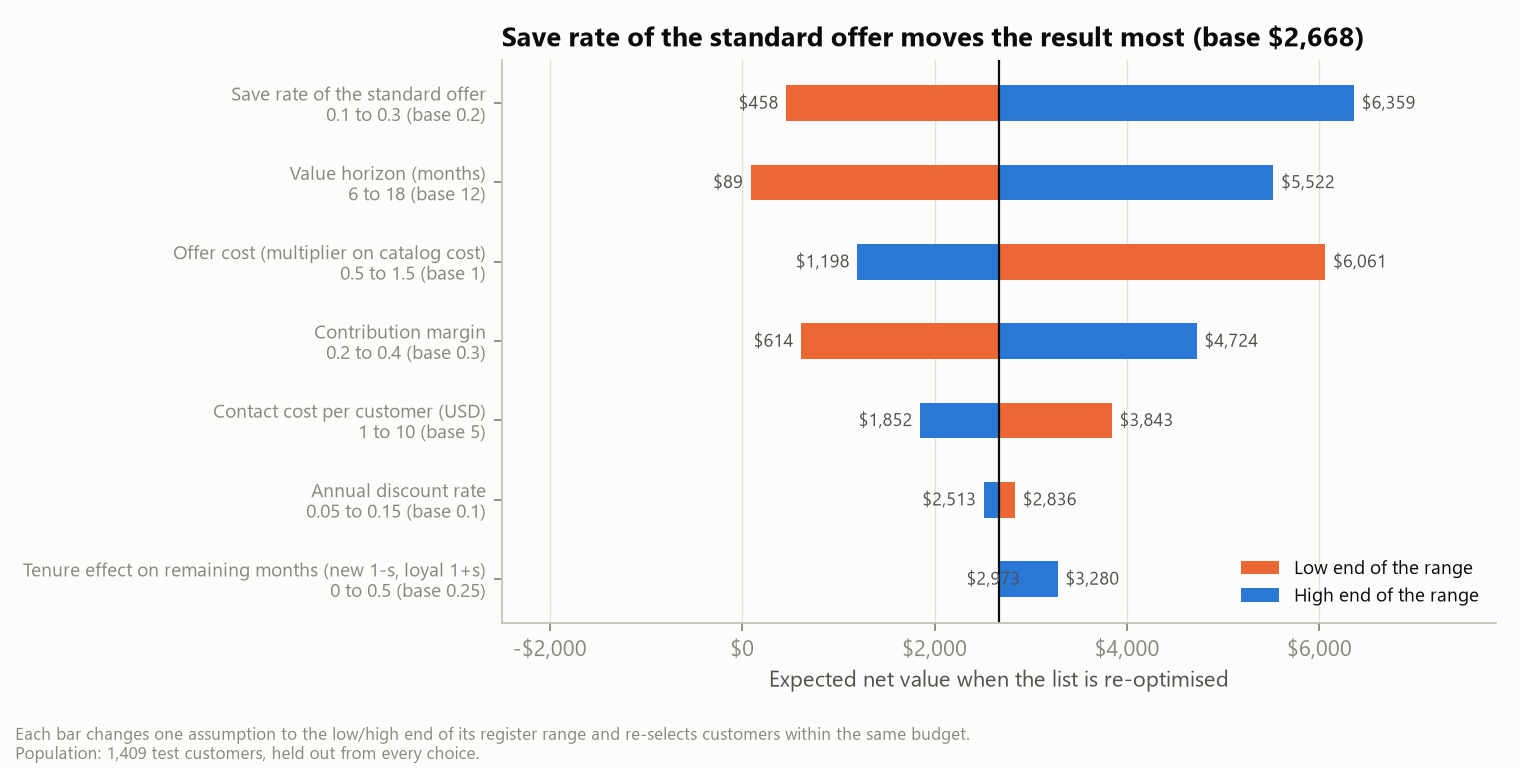
\includegraphics[width=0.49\linewidth]{tornado.png}\hfill
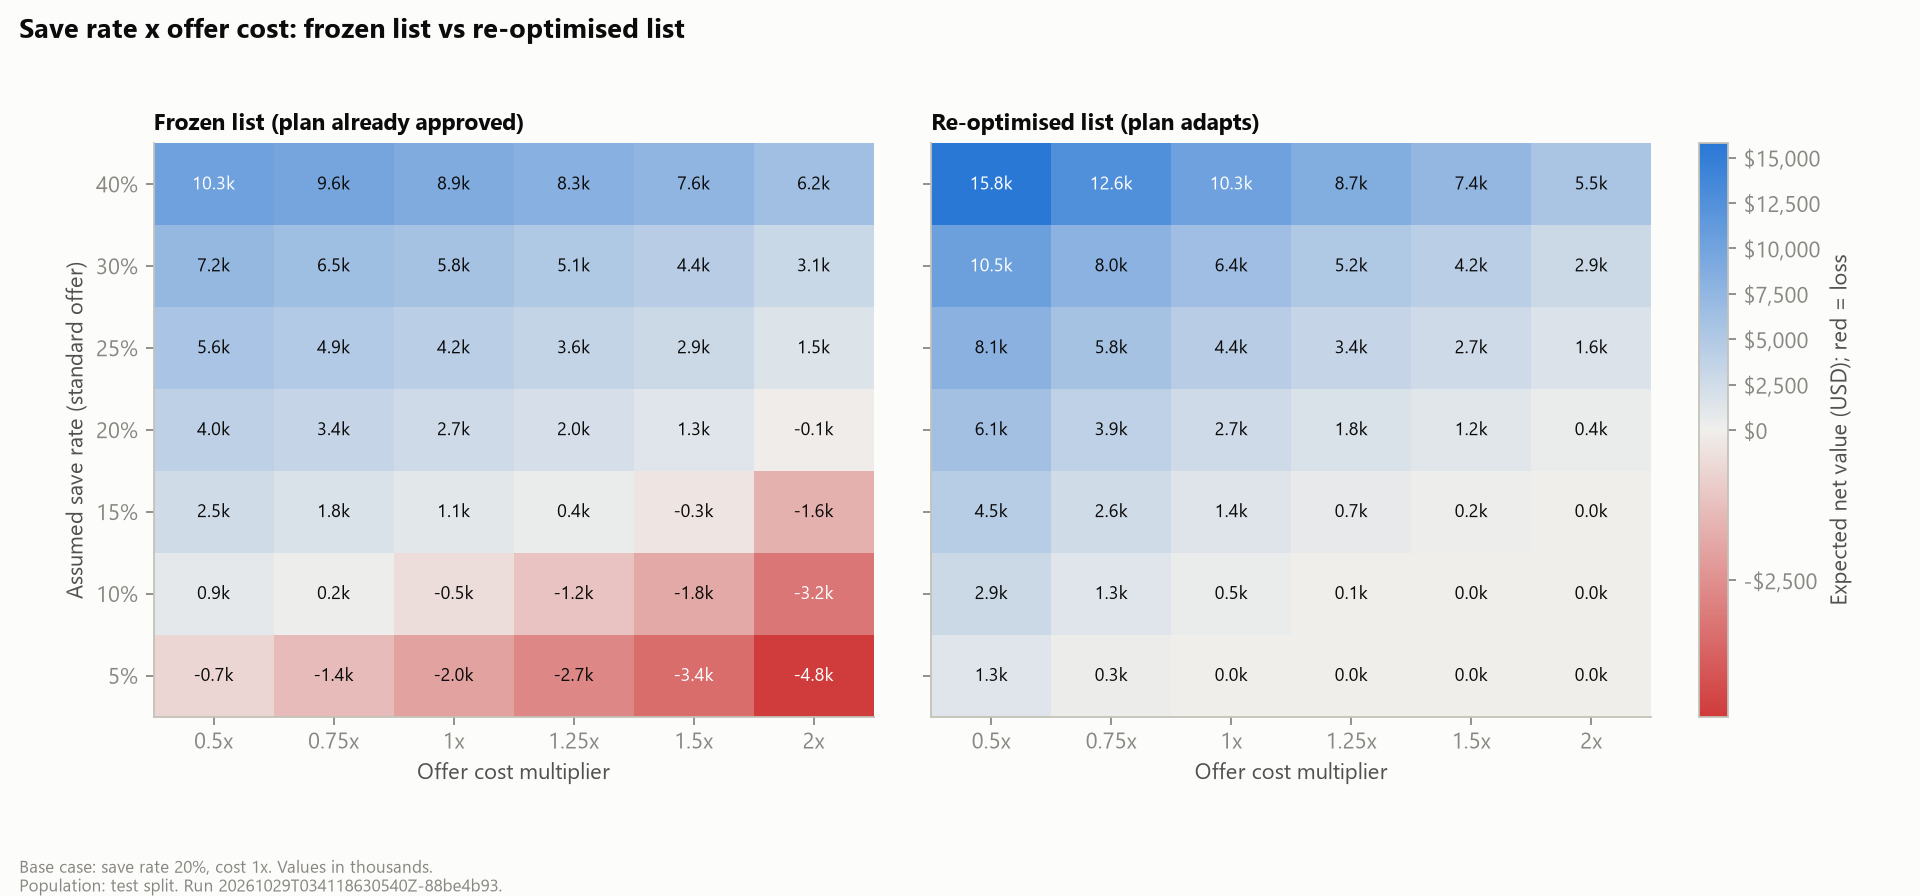
\includegraphics[width=0.49\linewidth]{sensitivity_heatmap.png}
\caption{Left: tornado chart. Right: save rate $\times$ offer cost grid, frozen and re-optimised lists.}
\label{fig:tornado}
\end{figure}

Over the save-rate $\times$ offer-cost grid the re-optimised plan ranges from \$0 to \$15,784, whereas a frozen list ranges from \textminus{}\$4,773 to \$10,311. A re-optimised plan can never lose money only because it pretends the true assumptions are known; a list that is actually sent can.

\textbf{Break-even.} The base-budget list breaks even at a standard-offer save rate of \textbf{11.3\%} or at offer costs 1.98$\times$ today's; the larger recommended list breaks even at \textbf{13.8\%}, because its additional customers have lower expected value. Both figures scale every offer's save rate in proportion and are expressed as the standard offer's rate; measured as the average save rate of the recommended offer mix, which is what a pilot observes, the break-even is 15.6\% against an assumed 22.6\%. Below a standard-offer save rate of 7.7\% no customer-offer pair has a positive EV and the right decision is not to run a campaign.

\begin{table}[H]
\centering\small
\caption{Combined scenarios (base budget).}\label{tab:scenarios}
\begin{tabularx}{\linewidth}{@{}lXrrr@{}}
\toprule
\textbf{Scenario} & \textbf{Assumptions} & \textbf{Contacted} & \textbf{Net (re-optimised)} & \textbf{Net (frozen)} \\
\midrule
Pessimistic & save rate 10\%, offer cost x1.25, contact cost \$8, margin 25\%, value horizon 9 months & 0 & \$0 & \textminus{}\$2,724 \\
Base & assumptions as registered & 153 & \$2,668 & \$2,668 \\
Optimistic & save rate 30\%, offer cost x0.75, contact cost \$2, margin 40\%, value horizon 15 months & 312 & \$19,084 & \$12,958 \\
\bottomrule
\end{tabularx}
\end{table}

\subsection{All assumptions uncertain at once}

The Monte Carlo analysis draws every register assumption at once from a triangular distribution over its range (mode at the base value), 5,000 times, and reprices the frozen lists (Table~\ref{tab:mc}, Figure~\ref{fig:mc}). A frozen list is repriced at the drawn costs, so when offers turn out dearer it spends more than its budget, as a list already sent would; the re-optimised comparison always stays within the budget.

\begin{table}[H]
\centering\small
\caption{Monte Carlo of all assumptions (5,000 draws, frozen lists, test split).}\label{tab:mc}
\begin{tabularx}{\linewidth}{@{}Lrrrrr@{}}
\toprule
\textbf{List} & \hd{Mean net} & \hd{5th pct.} & \hd{Median} & \hd{95th pct.} & \hd{P(loss)} \\
\midrule
Base-budget list & \$2,593 & \textminus{}\$469 & \$2,375 & \$6,282 & 9\% \\
Recommended list & \$3,997 & \textminus{}\$2,444 & \$3,639 & \$11,532 & 17\% \\
Risk-only list & \$1,241 & \textminus{}\$1,267 & \$1,080 & \$4,304 & 24\% \\
\bottomrule
\end{tabularx}
\end{table}

\begin{itemize}
  \item The recommended list earns more on average but is more exposed: it loses money in 17\% of draws against 9\% for the smaller base-budget list.
  \item Against the risk-only list at the same budget, expected-value targeting earns more in 99.96\% of draws (median gain \$1,240): \textbf{who to target is robust; how much an offer saves is not.}
  \item Value horizon (months), save rate of the standard offer and contribution margin drive most of the spread (rank correlations 0.59, 0.51, 0.42).
  \item Knowing the true assumptions before sending a list would be worth about \$846 per campaign of this size (\$4,227 across the base). This is the value of the information a pilot buys, and it recurs with every later wave.
\end{itemize}

\begin{figure}[H]
\centering
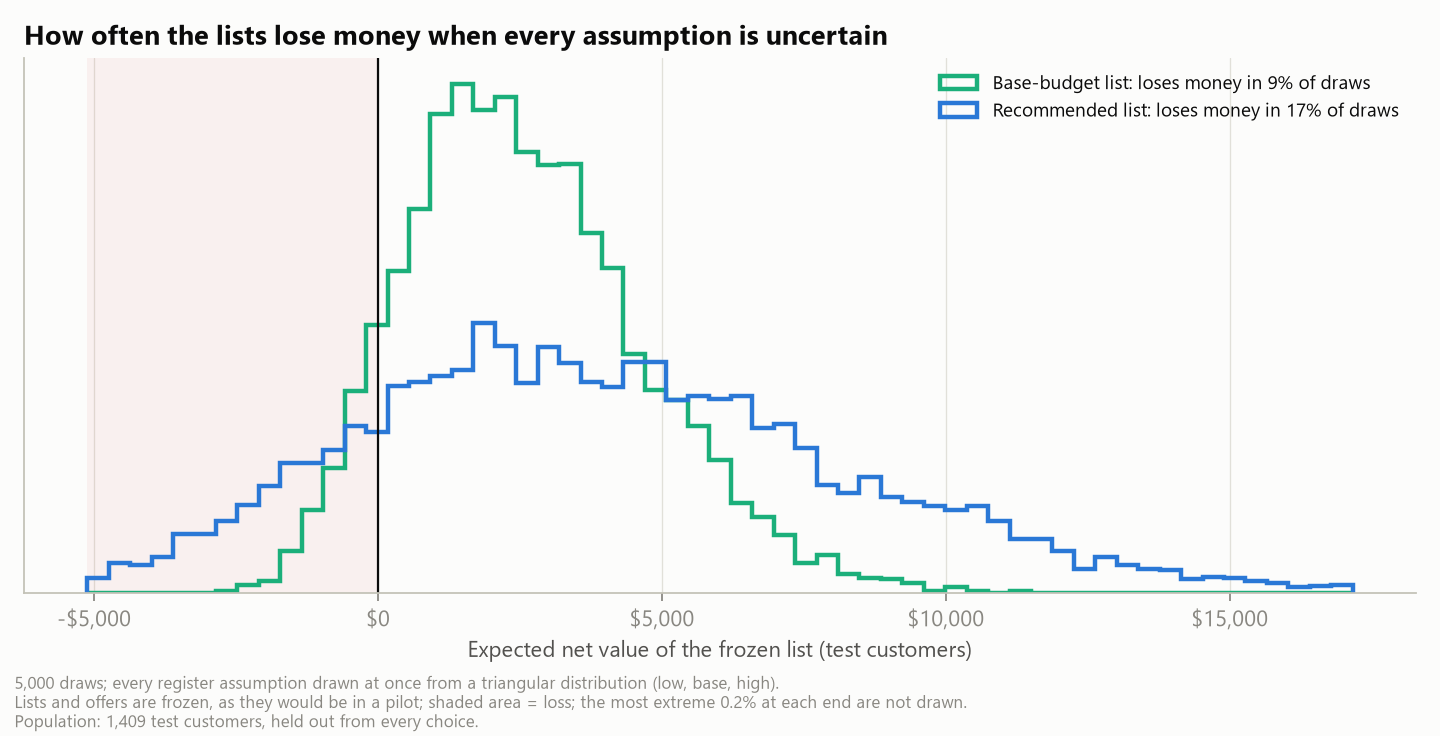
\includegraphics[width=0.8\linewidth]{monte_carlo.png}
\caption{Distribution of net value when all assumptions vary at once. Shaded area: loss.}
\label{fig:mc}
\end{figure}

\subsection{Outside the sample: lower churn and Vietnamese prices}

The sample's 27\% churn is far above that of real operators (US carriers report about 1\% monthly postpaid churn \cite{att2026,verizon2026}). To show what that does to the answer, all predicted probabilities were shifted by one constant on the log-odds scale until the average churn fell to 15\%, 10\%, 5\%, a prior-shift adjustment in the spirit of \cite{saerens2002}, with the constant chosen so that the average equals the target; the ranking of customers is unchanged. A second set of rows prices the same customers like a Vietnamese home-fibre operator (a 250,000 VND bill, about \$9.76; offers scaled to the same share of the bill; contact by one SMS of 500 VND).

\begin{table}[H]
\centering\small
\caption{Stress test without a budget limit. Worth an offer: customers with at least one positive-EV offer; expected net: the campaign under the contact cap.}\label{tab:stress}
\begin{tabularx}{\linewidth}{@{}Lrrrrr@{}}
\toprule
\textbf{Prices} & \hd{Average\\churn} & \hd{Worth an\\offer} & \hd{Share} & \hd{Expected net\\(USD)} & \hd{Pilot size\\per arm} \\
\midrule
Sample company (USD) & 27\% & 371 & 26\% & \$4,256 & 287 \\
Sample company (USD) & 15\% & 105 & 7\% & \$519 & 447 \\
Sample company (USD) & 10\% & 25 & 2\% & \$63 & 523 \\
Sample company (USD) & 5\% & 0 & 0\% & \$0 & n/a \\
Vietnam-like prices & 27\% & 463 & 33\% & \$948 & 304 \\
Vietnam-like prices & 15\% & 247 & 18\% & \$205 & 525 \\
Vietnam-like prices & 10\% & 98 & 7\% & \$48 & 689 \\
Vietnam-like prices & 5\% & 5 & 0\% & \$0 & 916 \\
\bottomrule
\end{tabularx}
\end{table}

Lower churn shrinks the target list fast: at 15\% average churn only 7\% of customers are worth the standard offer (against 26\% in the sample). With Vietnamese prices the money per customer is small, but an SMS costs almost nothing, so 18\% of customers remain worth an offer at 15\% churn: \emph{cheap contact matters more than the offer}. The pilot must also grow, from 287 customers per arm to 447 at 15\% churn.

% ================================================================ 9
\section{Fairness, Ethics and Customer Experience}

Gender and age are not model inputs, but they are used to audit \emph{who receives offers} \cite{barocas2023}. Selection-rate ratios outside 0.8--1.25 (the ``four-fifths'' screening analogy \cite{cfr1607}) are flagged for human review rather than corrected automatically (Figure~\ref{fig:fair}).

\begin{itemize}
  \item \textbf{Senior citizens} are contacted 3.34$\times$ as often as other customers under the recommended rule (2.64$\times$ under risk-only targeting). Adjusted for risk decile the ratio falls to 1.65$\times$: higher churn risk explains part of the gap and higher bills (value) the rest. Being selected means receiving both a discount and a call, so the gap is a benefit and a burden at once; it is flagged for review by Legal/DPO in every wave.
  \item \textbf{Gender:} ratio 1.15$\times$ (95\% interval 0.85--1.58), within normal variation.
  \item \textbf{Loyalty penalty:} long-tenure and contract customers are rarely contacted because their risk is low. To avoid the perception that only those who threaten to leave are rewarded \cite{cma2020}, the playbook recommends a non-targeted loyalty benefit funded outside the retention budget.
  \item \textbf{Contact burden and compliance:} at most 30\% of customers per wave, one retention contact per 30 days, consent and do-not-call checks; in Vietnam, advertising calls are limited to 08:00--17:00 and one per subscriber per 24 hours \cite{decree91}, and personal data processing requires purpose-specific consent \cite{pdpl2025}.
\end{itemize}

\begin{figure}[H]
\centering
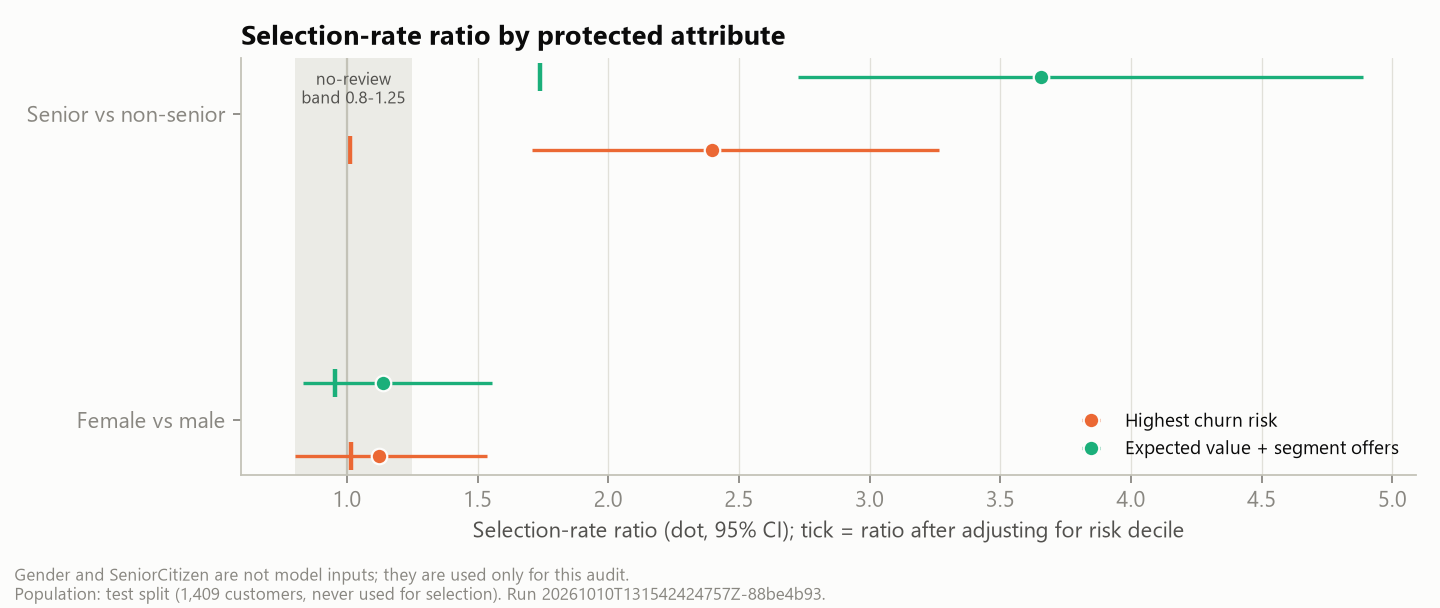
\includegraphics[width=0.8\linewidth]{fairness.png}
\caption{Selection rate by group relative to the reference group, for each targeting rule.}
\label{fig:fair}
\end{figure}

% ================================================================ 10
\section{Deployment: Dashboard and Pilot}

\subsection{Management dashboard}

A Streamlit dashboard (\texttt{app/Home.py}) turns the analysis into a decision tool, following the course's dashboard principles: one question per page, the key numbers top-left, colour used only for meaning. The \emph{Decision} page\IfFileExists{images/dashboard-decision.png}{ (Figure~\ref{fig:dash})}{} answers ``which customers should get an offer?'' with five KPIs: expected net value (with the gap to risk-only), ROI, customers contacted, precision among contacted and high-risk/high-value coverage. It also shows a one-sentence recommendation, who is and is not on the list, and an exportable action list with the reason for every decision. Budget and offer policy are inputs; the \emph{Assumptions \& sensitivity} page exposes every assumption, the break-even save rate, the live chance of a loss and the stress test; the \emph{Model evidence} page shows performance, the scorecard and the SHAP challenger, and scores uploaded customer files. The default view reproduces the numbers in this report exactly (same scenario ID).

\IfFileExists{images/dashboard-decision.png}{%
\begin{figure}[H]
\centering
\fbox{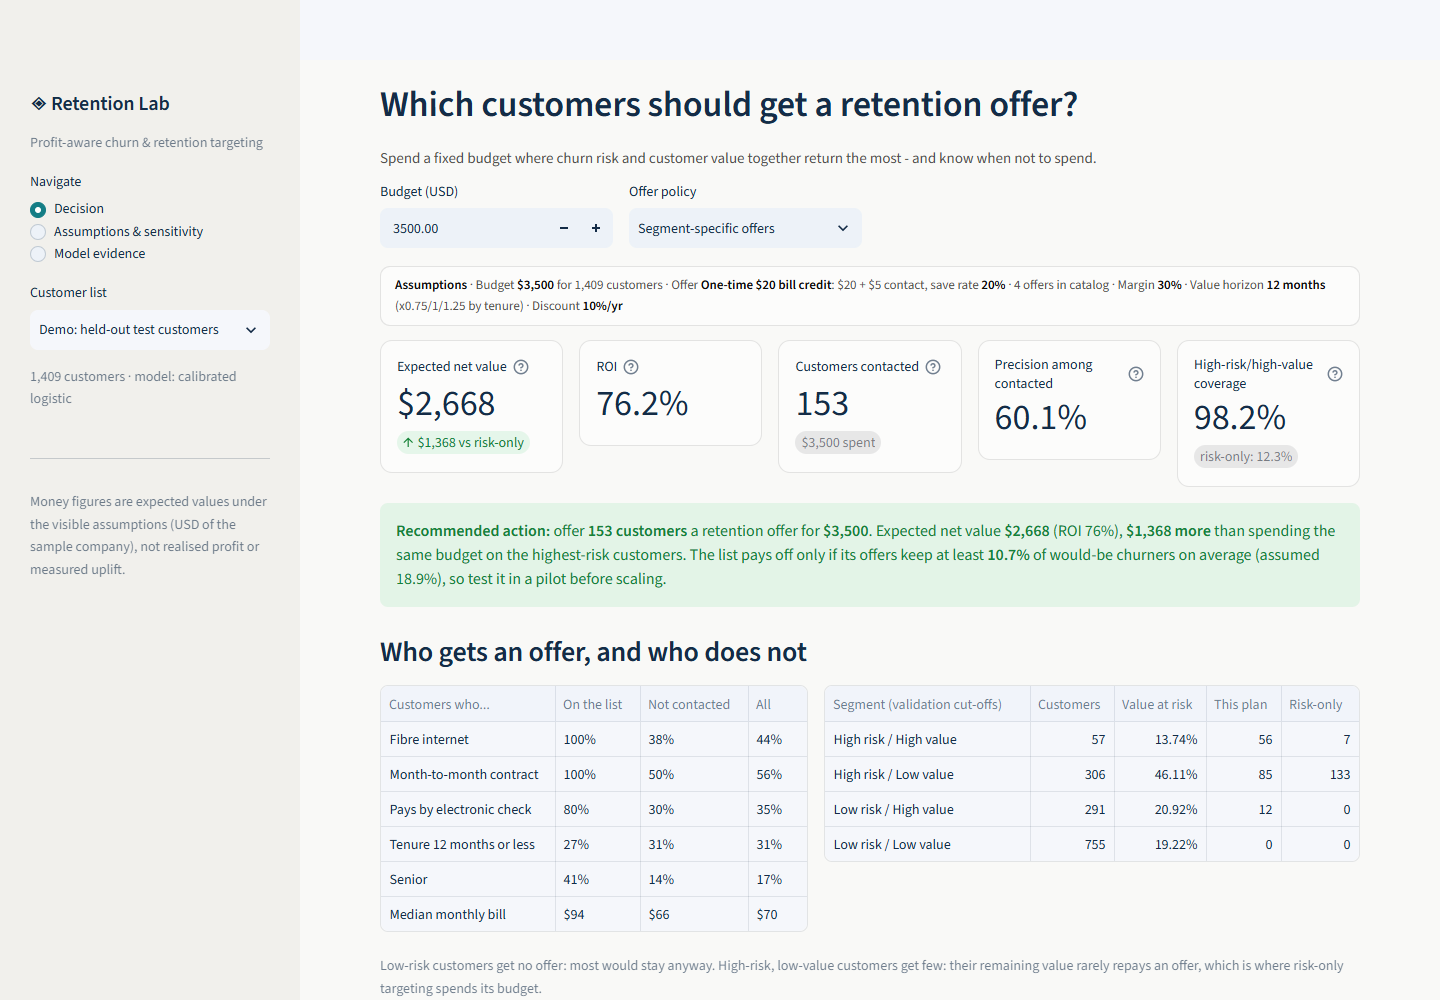
\includegraphics[width=0.9\linewidth]{dashboard-decision.png}}
\caption{Decision page of the dashboard (default assumptions, held-out test customers).}
\label{fig:dash}
\end{figure}}{}

\subsection{Randomised pilot}

Because the save rate cannot be estimated from these data, the recommendation is deployed as an experiment \cite{kohavi2020,ascarza2018}. One wave of 1,620 customers selected by the recommended rule is split at random: 810 receive the offer and 810 are held out. The save rate is the relative reduction of churn in the offered half against the held-out half after 90 days. Because the offered half receives a mix of offers, this measures the mix's average save rate, assumed to be 22.6\%; the list breaks even at 15.6\% on this scale.

\begin{itemize}
  \item \textbf{Power.} With 5\% significance and 80\% power, detecting the assumed 22.6\% save rate needs 213 customers per arm, and detecting the break-even rate (15.6\%) needs 447; one wave of 810 per arm covers both.
  \item \textbf{Decision rule, agreed in advance:} go if the 95\% interval of q is above 0 and q >= break-even; stop if q <= 0 or the interval is below break-even; otherwise extend (q = 1 - churn(offered) / churn(holdout), the list's mix save rate); at most 2 extra waves. If the true save rate is the assumed 22.6\%, the rule says ``go'' with probability 97\%.
  \item \textbf{Cost and downside:} offer and contact cost about \$22,875 for the offered half, expected net value \$10,363, worst case (nobody saved) \textminus{}\$22,875. A decision is available about 19 weeks after approval.
\end{itemize}

\begin{table}[H]
\centering\small
\caption{Roadmap from approval to scale-up.}\label{tab:roadmap}
\begin{tabularx}{\linewidth}{@{}lrp{3.6cm}X@{}}
\toprule
\textbf{Phase} & \textbf{Weeks} & \textbf{Owner} & \textbf{Work} \\
\midrule
Set-up & 4 & Retention, Legal/DPO, IT & consent and Do-Not-Call checks, data-protection impact assessment, CRM list export, call script and agent training \\
Pilot wave & 13 & Call centre, Retention & contact the offered half once; follow both halves for the 90-day outcome window \\
Read-out & 2 & Retention analytics & save rate with its interval, net value per customer, guardrail metrics; go, extend or stop \\
Scale or stop & 4 & Head of Retention, Finance & retrain and recalibrate on own data, replace assumed save rates, roll out the recommended budget \\
\bottomrule
\end{tabularx}
\end{table}

% ================================================================ 11
\section{Limitations and External Validity}

\begin{enumerate}
  \item \textbf{No causal uplift.} The data contain no randomised campaign, so save rates are assumptions and no uplift is claimed. High-risk customers may be the least responsive, and proactive contact can even raise churn \cite{ascarza2016,ascarza2018}. The pilot is designed to measure this; after several waves, uplift models can replace the save-rate assumption \cite{devriendt2021}.
  \item \textbf{Teaching sample.} A fictional US company with 27\% churn, far above real operators; IBM describes the churn window inconsistently (month vs quarter). The results demonstrate a method; their magnitudes do not transfer.
  \item \textbf{Snapshot and random split.} No dates, hence no temporal validation and no drift estimate; features are observed in the same snapshot as the label. Real deployment requires a time-based split and monitoring.
  \item \textbf{Value proxy.} No cost-to-serve, no re-churn after a save, no network effects; margin and horizon are assumptions and drive most of the uncertainty.
  \item \textbf{Label-based checks} reuse the assumed save rate. They validate \emph{who} is targeted, not \emph{whether offers work}.
  \item \textbf{Vietnamese context.} About 90\% of Vietnamese mobile subscriptions are prepaid \cite{sggp2022}, so churn appears as inactivity or number porting and contract features do not exist; the model must be rebuilt on operator data.
\end{enumerate}

% ================================================================ 12
\section{Conclusion and Recommendations}

Risk alone is the wrong criterion for spending a retention budget. A calibrated churn model, a transparent value proxy and an explicit expected-value rule select customers whose saved margin repays the offer, and at the same budget this delivers +\$1,368 (105\%) more expected value than calling the riskiest customers. The ranking advantage is robust to every assumption we tested; the absolute payoff is not, because it depends on a save rate nobody has measured.

\textbf{Recommendations to the Head of Retention:}
\begin{enumerate}
  \item Adopt expected-value targeting with segment offers for the next wave, at the recommended budget (\$6.49 per customer in the base).
  \item Run it as a randomised pilot of 1,620 customers, half held out, 90-day outcome; go only if the effect is significant and the save rate is at least 15.6\%.
  \item Replace the assumed save rates, margin and costs with measured values and re-run the pipeline; retrain on the operator's own data with a time-based split.
  \item Log customers' reasons for leaving and act on service problems (42\% of churners cite attitude or dissatisfaction), which no offer budget fixes.
  \item Operate under the guardrails: contact cap, consent, fairness review of every wave, and a non-targeted loyalty benefit.
\end{enumerate}

% ---------------------------------------------------------------- references
\begin{thebibliography}{99}\small
\bibitem{kaggle2018} BlastChar (2018). \emph{Telco Customer Churn} [data set, version 1]. Kaggle. \url{https://www.kaggle.com/datasets/blastchar/telco-customer-churn}
\bibitem{kaggle2020ibm} TanKY (2020). \emph{Telco customer churn: IBM dataset} [data set; IBM Cognos Analytics 11.1.3+ sample]. Kaggle. \url{https://www.kaggle.com/datasets/yeanzc/telco-customer-churn-ibm-dataset}
\bibitem{neslin2006} Neslin, S.~A., Gupta, S., Kamakura, W., Lu, J., \& Mason, C.~H. (2006). Defection detection: Measuring and understanding the predictive accuracy of customer churn models. \emph{Journal of Marketing Research}, 43(2), 204--211.
\bibitem{verbeke2012} Verbeke, W., Dejaeger, K., Martens, D., Hur, J., \& Baesens, B. (2012). New insights into churn prediction in the telecommunication sector: A profit driven data mining approach. \emph{European Journal of Operational Research}, 218(1), 211--229.
\bibitem{ascarza2018} Ascarza, E. (2018). Retention futility: Targeting high-risk customers might be ineffective. \emph{Journal of Marketing Research}, 55(1), 80--98.
\bibitem{ascarza2016} Ascarza, E., Iyengar, R., \& Schleicher, M. (2016). The perils of proactive churn prevention using plan recommendations: Evidence from a field experiment. \emph{Journal of Marketing Research}, 53(1), 46--60.
\bibitem{devriendt2021} Devriendt, F., Berrevoets, J., \& Verbeke, W. (2021). Why you should stop predicting customer churn and start using uplift models. \emph{Information Sciences}, 548, 497--515.
\bibitem{kohavi2020} Kohavi, R., Tang, D., \& Xu, Y. (2020). \emph{Trustworthy Online Controlled Experiments: A Practical Guide to A/B Testing}. Cambridge University Press.
\bibitem{gupta2004} Gupta, S., Lehmann, D.~R., \& Stuart, J.~A. (2004). Valuing customers. \emph{Journal of Marketing Research}, 41(1), 7--18.
\bibitem{faderhardie2014} Fader, P.~S., \& Hardie, B.~G.~S. (2014). \emph{What's wrong with this CLV formula?} \url{http://brucehardie.com/notes/033/}
\bibitem{platt1999} Platt, J.~C. (1999). Probabilistic outputs for support vector machines and comparisons to regularized likelihood methods. In \emph{Advances in Large Margin Classifiers}, 61--74. MIT Press.
\bibitem{niculescu2005} Niculescu-Mizil, A., \& Caruana, R. (2005). Predicting good probabilities with supervised learning. In \emph{Proceedings of ICML 2005}, 625--632.
\bibitem{guo2017} Guo, C., Pleiss, G., Sun, Y., \& Weinberger, K.~Q. (2017). On calibration of modern neural networks. In \emph{Proceedings of ICML 2017}, PMLR 70, 1321--1330.
\bibitem{vancalster2019} Van Calster, B., McLernon, D.~J., van Smeden, M., Wynants, L., \& Steyerberg, E.~W. (2019). Calibration: the Achilles heel of predictive analytics. \emph{BMC Medicine}, 17, 230.
\bibitem{saito2015} Saito, T., \& Rehmsmeier, M. (2015). The precision-recall plot is more informative than the ROC plot when evaluating binary classifiers on imbalanced datasets. \emph{PLOS ONE}, 10(3), e0118432.
\bibitem{lundberg2017} Lundberg, S.~M., \& Lee, S.-I. (2017). A unified approach to interpreting model predictions. In \emph{Advances in Neural Information Processing Systems 30}.
\bibitem{saerens2002} Saerens, M., Latinne, P., \& Decaestecker, C. (2002). Adjusting the outputs of a classifier to new a priori probabilities: A simple procedure. \emph{Neural Computation}, 14(1), 21--41.
\bibitem{barocas2023} Barocas, S., Hardt, M., \& Narayanan, A. (2023). \emph{Fairness and Machine Learning: Limitations and Opportunities}. MIT Press.
\bibitem{cfr1607} Uniform Guidelines on Employee Selection Procedures, 29 C.F.R. \S\,1607.4(D) (1978).
\bibitem{cma2020} Competition and Markets Authority (2020). \emph{Loyalty penalty update}. GOV.UK.
\bibitem{att2026} AT\&T Inc. (2026). \emph{Form 8-K, Exhibit 99.1: Fourth-quarter 2025 results}. U.S. SEC.
\bibitem{verizon2026} Verizon Communications Inc. (2026). \emph{Form 8-K, Exhibit 99: Fourth-quarter 2025 financial results}. U.S. SEC.
\bibitem{decree91} Government of Vietnam (2020). \emph{Decree No.\ 91/2020/ND-CP on fighting spam messages, spam emails and spam calls}.
\bibitem{pdpl2025} National Assembly of Vietnam (2025). \emph{Law on Personal Data Protection No.\ 91/2025/QH15}.
\bibitem{sggp2022} Saigon Giai Phong newspaper (2022, June 18). Report on the share of postpaid subscriptions and mobile number portability in Vietnam (in Vietnamese).
\end{thebibliography}

% ================================================================ appendix
\appendix
\section{Reproducibility and Project Package}

\begin{table}[H]
\centering\small
\caption{Where each required component of the project package is.}\label{tab:package}
\begin{tabularx}{\linewidth}{@{}p{5.2cm}X@{}}
\toprule
\textbf{Required component} & \textbf{Location in the repository} \\
\midrule
Reproducible code and notebooks, README & \path{src/telco_retention/}, \path{notebooks/} (four notebooks), \path{README.md} \\
Data dictionary and source log & \path{docs/data-dictionary.md}, \path{docs/source-log.md}, \path{docs/cleaning-log.md} \\
Executive brief (max.\ 2 pages) & \path{reports/executive-brief.pdf} \\
Interactive dashboard & \path{app/Home.py} (Streamlit) \\
Model / analysis card & \path{docs/model-card.md} \\
Churn scorecard and targeting table & \path{reports/tables/scorecard.csv}, \path{reports/tables/targeting_recommended.csv}, \path{docs/churn-scorecard.md} \\
Retention playbook & \path{docs/retention-playbook.md}, \path{docs/pilot-design.md} \\
Assumptions with sources & \path{configs/default.yaml}, \path{docs/assumption-register.md} \\
This report, the presentation and its script & \path{reports/final-report.pdf}, \path{reports/presentation/retention-presentation.pptx}, \path{reports/presentation/speaker-script.md} \\
\bottomrule
\end{tabularx}
\end{table}

\textbf{How to reproduce.} With Python 3.13:
\begin{quote}\small\ttfamily
python -m venv .venv\\
.venv\textbackslash Scripts\textbackslash python -m pip install -r requirements.lock.txt\\
.venv\textbackslash Scripts\textbackslash python -m pip install --no-deps -e .\\
.venv\textbackslash Scripts\textbackslash python -m telco\_retention run-all\\
.venv\textbackslash Scripts\textbackslash python -m streamlit run app/Home.py
\end{quote}
Each run is stored under \texttt{artifacts/runs/<run id>} with its configuration, data checksum, dependency versions and code hashes. The automated test suite (\texttt{pytest}) covers data validation, the model, the decision engine (including the optimiser against brute force), the analysis, the reports and the dashboard; a release script verifies that two independent runs produce identical metrics, customer lists and scenario identifiers.

\section{Final Submission Checklist}

\begin{table}[H]
\centering\small
\caption{Course checklist and where it is satisfied.}\label{tab:checklist}
\begin{tabularx}{\linewidth}{@{}Xp{6.4cm}@{}}
\toprule
\textbf{Checklist item} & \textbf{Evidence} \\
\midrule
Business decision, unit of analysis, target and evaluation period defined & Section 2, Table~\ref{tab:doc} \\
Source, download date, licence and filtering/joining documented & Section 3.1--3.2, \texttt{docs/source-log.md} \\
No target leakage; predictors available at decision time & Section~\ref{sec:leakage}, Table~\ref{tab:leak} \\
Baseline complete and compared fairly with advanced models & Section 5, Tables~\ref{tab:ablation}--\ref{tab:test} \\
Validation matches the structure of the problem & Section 3.4 (snapshot data: stratified split, test used once) \\
Technical metrics and a business metric reported & Sections 5 and 7 \\
Scenario assumptions visible, with sensitivity analysis & Section~\ref{sec:assumptions} \\
Dashboard supports a concrete decision & Section 10.1 \\
Executive brief states recommendation, impact range, risks, limitations & \texttt{reports/executive-brief.pdf}; Executive Summary \\
A third party can rerun the analysis & Appendix A \\
\bottomrule
\end{tabularx}
\end{table}

\section{Team Contributions}

\begin{table}[H]
\centering\small
\caption{Contributions of the members of Group 1.}\label{tab:team}
\begin{tabularx}{\linewidth}{@{}p{3.6cm}p{2.4cm}X@{}}
\toprule
\textbf{Member} & \textbf{Student ID} & \textbf{Main contributions} \\
\midrule
Pham Tuan Kiet & 20252751M & Code review and reproducibility check; final report and presentation slides \\
Nguyen Trung Hieu & 20261059M & Decision engine, robustness and Monte Carlo analysis, dashboard redesign, business documents \\
Bui Tien Dung & 20261204M & Review and quality assurance of code, report and slides \\
Pham Hung Phong & 20261061M & Data pipeline, churn models and first version of the dashboard \\
\bottomrule
\end{tabularx}
\end{table}

\end{document}
